% ============================================================
% Chapter 6 – Pickup-and-Delivery Problems for Goods Transportation
% Vehicle Routing: Problems, Methods, and Applications, 2nd ed. (2014)
% Self-contained Beamer slides
% ============================================================
\documentclass[aspectratio=169,10pt]{beamer}

\usetheme{Madrid}
\usecolortheme{seahorse}

\usepackage{amsmath,amssymb,amsthm}
\usepackage{booktabs}
\usepackage{array}
\usepackage{graphicx}
\usepackage{listings}
\usepackage{xcolor}
\usepackage{tikz}
\usepackage{pgfplots}
\pgfplotsset{compat=1.18}
\usepackage{microtype}
\usepackage{hyperref}
\usepackage{multicol}
\usepackage{tabularx}

\graphicspath{{figures/}}

\lstset{
  language=Python,
  basicstyle=\ttfamily\scriptsize,
  numbers=left,
  numberstyle=\tiny\color{gray},
  frame=single,
  backgroundcolor=\color{gray!7},
  commentstyle=\color{green!50!black}\itshape,
  keywordstyle=\color{blue!80!black}\bfseries,
  stringstyle=\color{orange!80!black},
  breaklines=true,
  showstringspaces=false,
  tabsize=4,
  xleftmargin=2em,
  numbersep=6pt,
}

\setbeamertemplate{footline}[frame number]
\setbeamertemplate{navigation symbols}{}

% ── Title ──────────────────────────────────────────────────
\title[Chapter 6: PDP for Goods]{%
  Chapter 6: Pickup-and-Delivery Problems\\for Goods Transportation}
\subtitle{Vehicle Routing: Problems, Methods, and Applications\\
  Second Edition, 2014}
\author[Battarra, Cord\'{e}au, Iori]{%
  Maria Battarra \and Jean-Fran\c{c}ois Cord\'{e}au \and Manuel Iori}
\date{Chapter 6, pp.\ 161--202}

% ============================================================
\begin{document}
% ============================================================

\begin{frame}
  \titlepage
\end{frame}

% ── Table of contents ──────────────────────────────────────
\begin{frame}[allowframebreaks]{Chapter Outline}
  \tableofcontents
\end{frame}

% ============================================================
\section{Introduction}
% ============================================================

\begin{frame}[allowframebreaks]{6.1 Introduction: What Are Pickup-and-Delivery Problems?}

  Pickup-and-Delivery Problems (PDPs) constitute an important and broad family of routing
  problems in which goods or passengers must be transported between origins and destinations.
  Unlike the classical Vehicle Routing Problem (VRP) -- in which goods flow only \emph{from}
  a depot \emph{to} customers -- a PDP involves two-sided requests: for each request there is
  a \textbf{pickup location} where the item is collected and a \textbf{delivery location} where
  the item is dropped off.

  \begin{block}{Formal Definition of a PDP Request}
    A \textbf{request} $r$ specifies:
    \begin{itemize}
      \item a \textbf{pickup node} $p_r$: the origin where the item must be collected,
      \item a \textbf{delivery node} $d_r$: the destination where the item must be delivered,
      \item a \textbf{load} $q_r$: the quantity (weight, volume) associated with the request,
      \item (optionally) \textbf{time windows} $[e_{p_r}, l_{p_r}]$ and $[e_{d_r}, l_{d_r}]$
            specifying the earliest and latest service times at both endpoints.
    \end{itemize}
    The fundamental constraint is that the pickup must occur \emph{before} the delivery on
    the same vehicle's route.
  \end{block}

  \framebreak

  \textbf{Three structural categories.} PDPs are classified according to the relationship
  between origins and destinations of requests:

  \begin{enumerate}
    \item \textbf{Many-to-Many (M-M):} Any node can be both an origin and a destination.
          This arises in transportation networks such as freight exchange platforms, where
          goods move between arbitrary pairs of nodes. Dial-a-ride problems without fixed
          depot constraints are special cases.

    \item \textbf{One-to-Many-to-One (1-M-1):} Goods originate from a \emph{single depot},
          are delivered to customers, and empty or loaded vehicles return to the same depot.
          This models distribution networks where a vehicle may also collect goods (e.g.,
          returned merchandise) during the same tour.

    \item \textbf{One-to-One (1-1):} Each request specifies a \emph{unique} pickup location
          and a \emph{unique} delivery location. Items cannot be transhipped: the same
          vehicle that picks up an item must deliver it. This is the most constrained and
          the most widely studied variant for goods transportation.
  \end{enumerate}

  \begin{figure}[h]
    \centering
    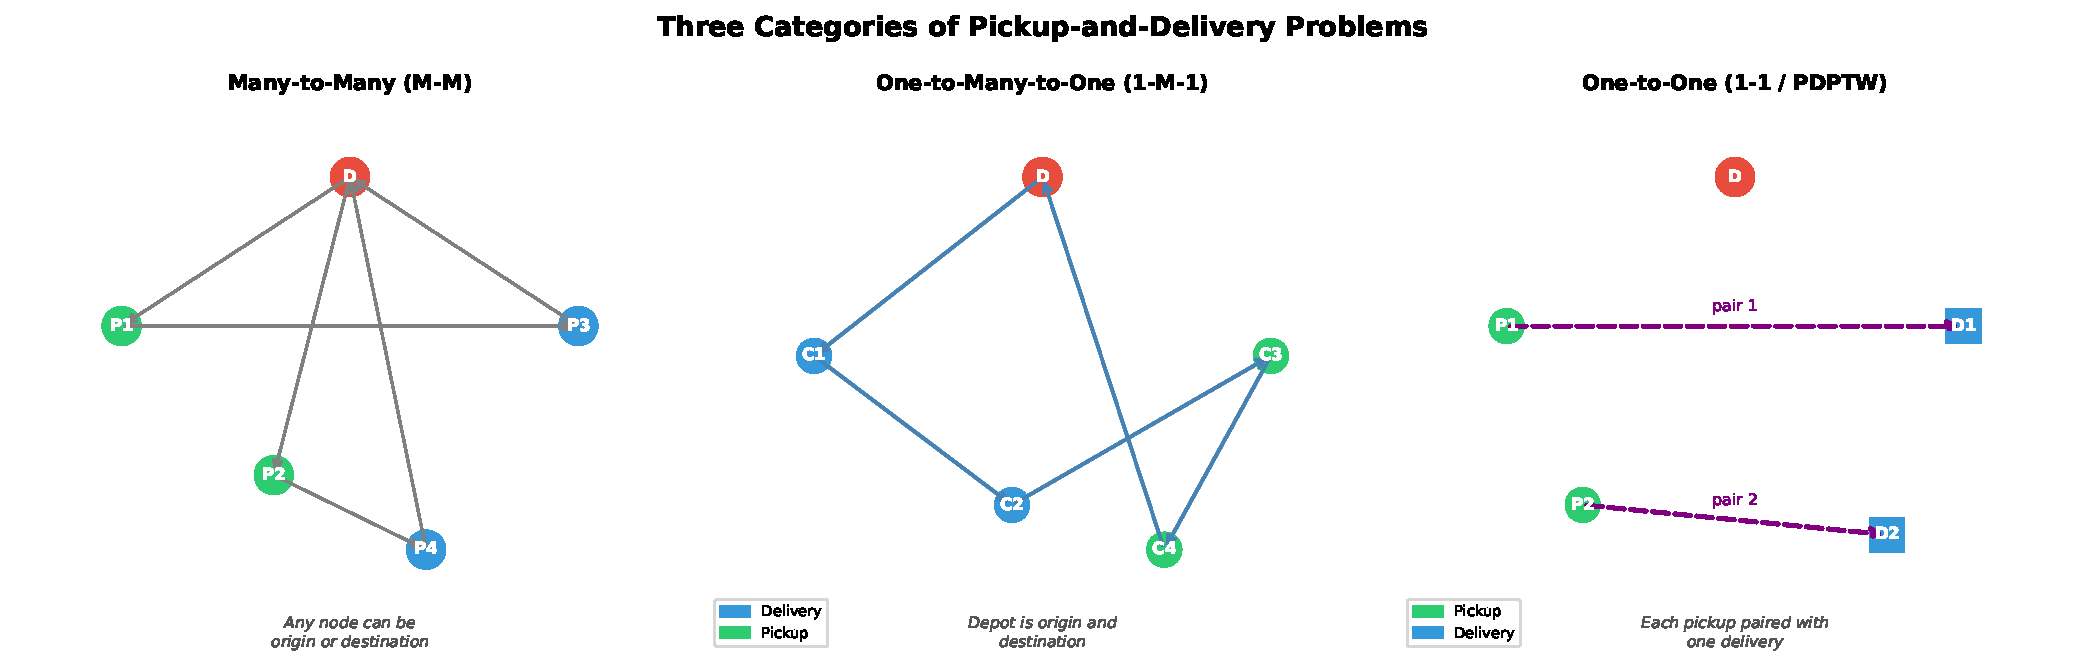
\includegraphics[width=0.95\textwidth]{fig_pdp_types.pdf}
    \caption{The three structural categories of PDPs. Green = pickup nodes, blue = delivery
      nodes, red = depot. In M-M any node is both; in 1-M-1 the depot is origin/destination;
      in 1-1 each pickup is paired with exactly one delivery.}
  \end{figure}

  \framebreak

  \textbf{Additional problem dimensions.} Beyond the structural category, PDPs are further
  characterised by:
  \begin{itemize}
    \item \textbf{Fleet composition:} homogeneous (all vehicles identical) or heterogeneous
          (vehicles differ in capacity, cost, or type).
    \item \textbf{Time windows:} hard (service outside the window is forbidden) or soft
          (violations are penalised in the objective).
    \item \textbf{Loading constraints:} LIFO (Last-In First-Out), FIFO (First-In First-Out),
          or full three-dimensional packing feasibility.
    \item \textbf{Objective:} minimise total travel distance or time, minimise number of
          vehicles, or a weighted combination.
  \end{itemize}

  \begin{alertblock}{Key Insight: Why PDPs Are Harder Than VRPs}
    In a standard VRP, feasibility checking for a route requires only that the total
    demand does not exceed capacity. In a PDP, feasibility also requires:
    (1) the pickup precedes its paired delivery (\emph{precedence} constraint),
    (2) the vehicle load never exceeds capacity at any point on the route (\emph{capacity}
    constraint along the tour, not just in total), and
    (3) all time windows are satisfied. The combination of these constraints makes PDPs
    significantly harder combinatorially.
  \end{alertblock}

  \textbf{Dynamic and stochastic variants.} Many real-world applications involve
  \emph{dynamic} PDPs in which requests arrive in real time (courier services, taxi
  dispatching), or \emph{stochastic} PDPs in which demand or travel times are uncertain.
  This chapter focuses on the static, deterministic setting.

\end{frame}

% ============================================================
\section{Many-to-Many Problems}
% ============================================================

\begin{frame}[allowframebreaks]{6.2 Many-to-Many (M-M) Problems}

  In the Many-to-Many PDP, multiple origins and multiple destinations exist, and any node
  can serve as both an origin and a destination. The classic example is a transportation
  network where goods are to be moved between arbitrary pairs of nodes, typically using
  a fleet of vehicles.

  \begin{block}{M-M PDP: Mathematical Formulation}
    Let $G = (V, A)$ be a directed graph where $V = \{0, 1, \ldots, n\}$ is the node set
    and $A$ is the arc set.  Each node $i \in V$ has a \textbf{supply} $s_i$ (positive if
    it produces goods, negative if it consumes goods).  We seek routes for $m$ vehicles
    of capacity $Q$ such that:
    \[
      \min \sum_{k=1}^{m} \sum_{(i,j) \in A} c_{ij} x_{ij}^k
    \]
    subject to flow conservation at every node, vehicle capacity constraints, and the
    requirement that all supply--demand imbalances are resolved.  Here $c_{ij}$ is the
    travel cost of arc $(i,j)$ and $x_{ij}^k \in \{0,1\}$ indicates whether vehicle $k$
    traverses arc $(i,j)$.
  \end{block}

  \textbf{Dial-a-Ride relaxation.} A well-known special case of M-M problems is the
  \textbf{Dial-a-Ride Problem (DARP)}, in which users specify an origin and destination
  and a vehicle must transport them. In the goods context, the ``passengers'' are replaced
  by freight units. When the depot is not a fixed constraint -- meaning vehicles may start
  and end at any node -- the problem becomes a pure M-M problem.

  \framebreak

  \textbf{Single-vehicle case.} Hernandez-Perez and Salazar-Gonzalez~(2004) introduced
  the \textbf{1-PDTSP} (one-vehicle Pickup-and-Delivery Travelling Salesman Problem) for
  M-M settings.  A complete graph $G = (V, A)$ is given; each node $i$ has a supply
  $s_i$ (positive = source, negative = sink), and a single vehicle of capacity $Q$
  must visit all nodes.  The 1-PDTSP can be formulated as:

  \begin{block}{1-PDTSP Formulation}
    \textbf{Decision variables:}
    \begin{itemize}
      \item $x_{ij} \in \{0,1\}$: equals 1 if arc $(i,j)$ is traversed by the vehicle.
      \item $y_i \geq 0$: vehicle load upon departure from node $i$.
    \end{itemize}
    \textbf{Objective:}
    \[
      \min \sum_{(i,j) \in A} c_{ij} x_{ij}
    \]
    \textbf{Constraints:}
    \begin{align}
      \sum_{j} x_{ij} &= 1 \quad \forall i \in V \tag{1: each node left once} \\
      \sum_{i} x_{ij} &= 1 \quad \forall j \in V \tag{2: each node entered once} \\
      y_j &\geq y_i + s_j \cdot x_{ij} - Q(1 - x_{ij}) \quad \forall i \neq j
            \tag{3: load tracking} \\
      0 &\leq y_i \leq Q \quad \forall i \in V \tag{4: capacity} \\
      x_{ij} &\in \{0,1\} \tag{5: binary}
    \end{align}
    \emph{Symbol glossary:} $c_{ij}$ = travel cost of arc $(i,j)$; $s_i$ = supply at
    node $i$ (negative for demand); $Q$ = vehicle capacity; $y_i$ = load leaving node $i$.
  \end{block}

  \framebreak

  \textbf{Interpretation of the load-tracking constraint.} Constraint~(3) ensures that
  when the vehicle travels from $i$ to $j$, the load $y_j$ upon departure from $j$ equals
  $y_i$ (load leaving $i$) plus $s_j$ (supply or demand at $j$).  When $x_{ij} = 0$ the
  constraint is relaxed by the big-$M$ term $Q(1-x_{ij})$, making it non-binding.  This
  classical technique for linearising product terms in integer programs is known as the
  \textbf{big-$M$ formulation}.

  \begin{exampleblock}{Worked Example: 1-PDTSP with 4 Nodes}
    Suppose we have nodes $\{0, 1, 2, 3\}$ with supplies $s_0 = 0$, $s_1 = +3$ (pickup),
    $s_2 = -3$ (delivery), $s_3 = +2$ (pickup), and a vehicle of capacity $Q = 5$.
    One feasible route is $0 \to 1 \to 3 \to 2 \to 0$:
    \begin{itemize}
      \item Load after visiting node 0: $y_0 = 0$.
      \item Load after visiting node 1: $y_1 = 0 + 3 = 3 \leq 5$. \checkmark
      \item Load after visiting node 3: $y_3 = 3 + 2 = 5 \leq 5$. \checkmark
      \item Load after visiting node 2: $y_2 = 5 - 3 = 2 \leq 5$. \checkmark
      \item Return to depot: load = 2 (note: demand at node 3 remains unsatisfied;
            a second vehicle or additional depot visit would be needed).
    \end{itemize}
    An \emph{infeasible} route would be $0 \to 3 \to 1 \to 2 \to 0$ only if capacity
    were exceeded: loads would be $0, 2, 5, 2$ -- still feasible here.  If $s_3 = +4$
    instead, the route $0 \to 1 \to 3 \to 2 \to 0$ would require load $= 3 + 4 = 7 > Q=5$
    at node 3, making it infeasible.
  \end{exampleblock}

  \framebreak

  \textbf{Exact algorithms for the 1-PDTSP.} The 1-PDTSP was introduced by Hernandez-Perez
  and Salazar-Gonzalez (2004), who provided a branch-and-cut algorithm with the separation
  of subtour elimination constraints.  They reported solving instances with up to 40 nodes
  optimally.  The proposed branch-and-cut utilises:
  \begin{itemize}
    \item Subtour-elimination constraints (SEC): these prevent the solution from containing
          disconnected sub-cycles, analogous to the Dantzig-Fulkerson-Johnson constraints
          for the TSP.
    \item Capacity cuts: valid inequalities that tighten the LP relaxation by exploiting
          load constraints.
  \end{itemize}

  \textbf{Heuristics for the 1-PDTSP.} Because the 1-PDTSP is NP-hard (it generalises
  the TSP), exact methods are impractical for large instances. Heuristic approaches include:
  \begin{itemize}
    \item \textbf{Greedy construction:} build the route by inserting nodes in order of
          most profitable contribution to the tour.
    \item \textbf{Local search:} apply or-opt moves (relocate a single node or a chain
          of consecutive nodes to a better position), 2-opt edge exchanges, and 3-opt moves.
    \item \textbf{Genetic algorithms:} use crossover operators that respect the
          feasibility structure of the 1-PDTSP.
    \item \textbf{VNS (Variable Neighbourhood Search):} systematically explore successively
          larger neighbourhoods to escape local optima.
  \end{itemize}

  \framebreak

  \textbf{Multiple vehicles: the M-PDTSP.} Qu and Bard~(2012) studied the M-M problem
  with multiple vehicles (M-PDTSP) and introduced an GRASP+VND metaheuristic. The
  algorithm has two phases:
  \begin{enumerate}
    \item \textbf{GRASP construction phase:} build an initial solution using a greedy
          randomised adaptive procedure that selects the next node with a probability
          proportional to a restricted candidate list (RCL) of the best insertions.
    \item \textbf{VND (Variable Neighbourhood Descent) improvement:} apply a sequence
          of local-search neighbourhoods -- including node relocation, pair relocation,
          and route merging -- until no improvement is found in any neighbourhood.
  \end{enumerate}
  This algorithm was tested on benchmark instances and showed competitive solutions
  compared to branch-and-cut methods, while being applicable to much larger instances.

  \begin{alertblock}{Key Takeaway: M-M Problems}
    Many-to-Many PDPs generalise both the TSP and the classical VRP. The single-vehicle
    variant (1-PDTSP) is NP-hard and requires branch-and-cut for exact optimisation.
    Metaheuristics such as GRASP with VNS or variable neighbourhood descent are the
    methods of choice for instances with more than about 40 nodes.
  \end{alertblock}

\end{frame}

% ============================================================
\section{One-to-Many-to-One Problems}
% ============================================================

\begin{frame}[allowframebreaks]{6.3 One-to-Many-to-One (1-M-1) Problems}

  In the One-to-Many-to-One PDP, all goods originate from (or return to) a single depot.
  Vehicles depart from the depot carrying goods for delivery, visit customers to make
  deliveries, and may also collect goods (pickups) from customers during the same tour
  before returning to the depot. This structure models real-world applications such as
  beverage distribution (delivering full crates and collecting empty ones), or the
  simultaneous distribution and collection of products in retail networks.

  \begin{figure}[h]
    \centering
    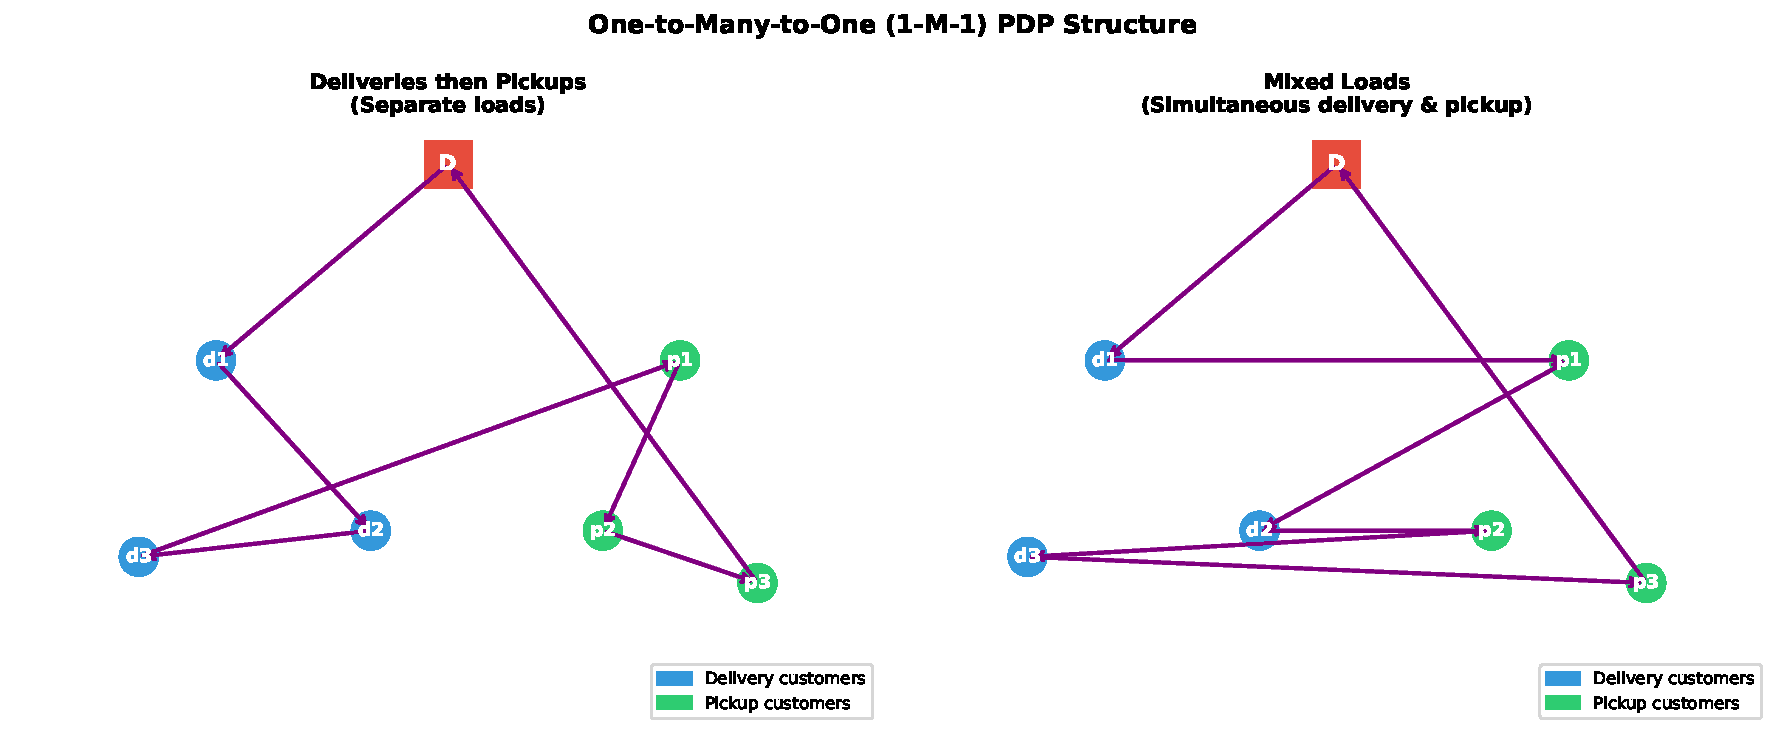
\includegraphics[width=0.80\textwidth]{fig_1m1_problem.pdf}
    \caption{Two variants of the 1-M-1 structure. Left: deliveries precede pickups
      (vehicles first unload all goods, then collect). Right: mixed loads (delivery and
      pickup customers are interleaved on the route).}
  \end{figure}

  \framebreak

  \textbf{Two sub-cases of 1-M-1.} The 1-M-1 structure can be further divided:
  \begin{enumerate}
    \item \textbf{Deliveries then pickups:} the vehicle visits all delivery customers
          before visiting any pickup customer. This is a natural operational constraint
          when delivery and pickup goods cannot be mixed (e.g., fragile items).
    \item \textbf{Mixed loads:} delivery and pickup customers are interleaved on the route.
          The vehicle load at any point is the original delivery load minus goods
          delivered plus goods collected up to that point. The capacity constraint must
          hold throughout the route.
  \end{enumerate}

  \begin{block}{The Vehicle Routing Problem with Simultaneous Pickup and Delivery (VRPSPD)}
    The VRPSPD is the most general form of 1-M-1.  A fleet of $m$ homogeneous vehicles,
    each of capacity $Q$, must serve $n$ customers.  Each customer $i$ has a
    \textbf{delivery demand} $d_i > 0$ and a \textbf{pickup demand} $p_i \geq 0$.
    The vehicle must carry both when visiting customer $i$.

    \medskip
    \textbf{Decision variables:}
    \begin{itemize}
      \item $x_{ij}^k \in \{0,1\}$: 1 if vehicle $k$ travels from $i$ to $j$.
      \item $y_{ij}^k \geq 0$: delivery load on vehicle $k$ when traversing arc $(i,j)$.
      \item $z_{ij}^k \geq 0$: pickup load on vehicle $k$ when traversing arc $(i,j)$.
    \end{itemize}

    \textbf{Objective -- minimise total travel cost:}
    \[
      \min \sum_{k=1}^{m} \sum_{(i,j) \in A} c_{ij} x_{ij}^k
    \]

    \textbf{Core constraints:} flow conservation, each customer visited exactly once,
    and at every arc the combined delivery and pickup loads must satisfy:
    \[
      y_{ij}^k + z_{ij}^k \leq Q \cdot x_{ij}^k \quad \forall i,j,k.
    \]
    This states that total load (unsatisfied deliveries + collected pickups) on any arc
    must not exceed vehicle capacity $Q$.
  \end{block}

  \framebreak

  \textbf{The Hamiltonian Delivery Problem (HDP).} A special sub-case introduced by
  Montane and Galvao~(2006) requires a vehicle to visit all customers on a single Hamiltonian
  route.  The HDP is equivalent to the VRPSPD with a single vehicle, and serves as a
  theoretical foundation for the general problem.

  \textbf{Exact methods for VRPSPD.} The problem is NP-hard, so exact methods can only
  handle small instances (typically $n \leq 25$ customers). Approaches include:
  \begin{itemize}
    \item \textbf{Branch-and-bound} with lower bounds derived from LP relaxations.
    \item \textbf{Branch-and-cut} using capacity constraints and subtour eliminators
          as cutting planes.
    \item \textbf{Set-partitioning formulations} solved via column generation, where
          each column is a feasible vehicle route.
  \end{itemize}

  \textbf{Construction heuristics.}  The most common approach is a \textbf{greedy insertion
  heuristic}: start with an empty route, and repeatedly insert the customer (and its
  delivery--pickup pair) at the position in the route that results in the smallest
  increase in total travel cost, subject to feasibility. This runs in $O(n^3)$ time
  for a single vehicle.

  \begin{exampleblock}{Worked Example: VRPSPD with 4 Customers, $Q = 10$}
    Customers: $d_1=3, p_1=2$;\ $d_2=2, p_2=4$;\ $d_3=1, p_3=3$;\ $d_4=4, p_4=1$.
    Vehicle starts at depot with load $= \sum d_i = 10$.  Route $0 \to 1 \to 2 \to 3 \to 4 \to 0$:
    \begin{center}
      \begin{tabular}{lcccc}
        \toprule
        \textbf{After visiting} & \textbf{Delivered} & \textbf{Collected} & \textbf{Load} & \textbf{Feasible?} \\
        \midrule
        Depot (start) & 0 & 0 & 10 & $\leq 10$ \checkmark \\
        Customer 1    & 3 & 2 & 9  & $\leq 10$ \checkmark \\
        Customer 2    & 2 & 4 & 11 & $> 10$ \textbf{X} \\
        \bottomrule
      \end{tabular}
    \end{center}
    Route $0\to1\to2\to3\to4\to0$ is \emph{infeasible} because after customer 2 the
    load is 11 (deliveries 3+2=5 done, pickups 2+4=6 collected: load = $10-5+6=11$).
    Reordering as $0\to1\to3\to4\to2\to0$: load sequence is $10, 9, 9, 6, 8$, all
    $\leq 10$. \checkmark
  \end{exampleblock}

  \framebreak

  \textbf{Metaheuristics for VRPSPD.}  Population-based and trajectory-based methods
  have both been applied with success:

  \begin{itemize}
    \item \textbf{Tabu Search (Montane \& Galvao, 2006):} maintains a tabu list of
          recently performed moves (node relocations, 2-opt exchanges) and forbids
          reversing them for a prescribed number of iterations, forcing exploration of
          new solution regions.
    \item \textbf{GRASP (Bianchessi \& Righini, 2007):} iterates between a greedy
          randomised construction phase and a local-search improvement phase.
    \item \textbf{Large Neighbourhood Search (LNS, Ropke \& Pisinger, 2006):}
          repeatedly removes a subset of customers from the current solution and
          reinserts them in a better position. The destroy operator may remove customers
          related by geography or time; the repair operator uses a greedy insertion.
    \item \textbf{Genetic Algorithm with B\&C (Goksal et al., 2013):} uses a parallel
          multi-population GA whose fitness evaluation calls a branch-and-cut sub-routine
          for local route improvement.
  \end{itemize}

  \textbf{Backhaul variants.}  When the constraint is imposed that \emph{all deliveries
  precede all pickups} on a route, the problem becomes the VRP with Backhauls (VRPB).
  This is less general than VRPSPD, since the mixed-load requirement is dropped, but
  it models many practical distribution scenarios (e.g., delivery trucks that also
  collect returns only after unloading all forward deliveries).

  \begin{alertblock}{Key Takeaway: 1-M-1 Problems}
    The VRPSPD extends the classical VRP by allowing each customer to both receive
    and send goods in a single visit. The critical complication relative to standard
    VRP is that feasibility must be checked at every arc of the route, not just
    in aggregate. LNS-based metaheuristics have emerged as the most effective
    general-purpose approach.
  \end{alertblock}

\end{frame}

% ============================================================
\section{One-to-One Problems}
% ============================================================

\begin{frame}[allowframebreaks]{6.4.1 The PDPTW: Mathematical Formulation}

  The \textbf{Pickup-and-Delivery Problem with Time Windows (PDPTW)} is the most extensively
  studied variant of the 1-1 PDP. In this problem, each request specifies a unique pickup
  location and a unique delivery location with associated time windows, and the same vehicle
  that picks up the goods must deliver them without intermediate transhipment.

  \textbf{Problem data.}
  \begin{itemize}
    \item $n$: number of requests.
    \item Node set: $N = \{0, 1, \ldots, 2n, 2n+1\}$ where node $0$ is the origin depot,
          node $2n+1$ is the destination depot (a copy of node 0), nodes $1, \ldots, n$ are
          pickup nodes, and nodes $n+1, \ldots, 2n$ are delivery nodes.
    \item Each request $i \in \{1, \ldots, n\}$ consists of pickup node $i$ and delivery
          node $n+i$.
    \item $c_{ij}$: travel cost from node $i$ to node $j$.
    \item $t_{ij}$: travel time from node $i$ to node $j$.
    \item $[e_i, l_i]$: time window at node $i$ (service must begin in this interval).
    \item $q_i$: load change at node $i$ ($q_i > 0$ for pickup nodes, $q_i < 0$ for delivery nodes).
    \item $Q$: vehicle capacity (maximum load at any point in the route).
  \end{itemize}

  \begin{figure}[h]
    \centering
    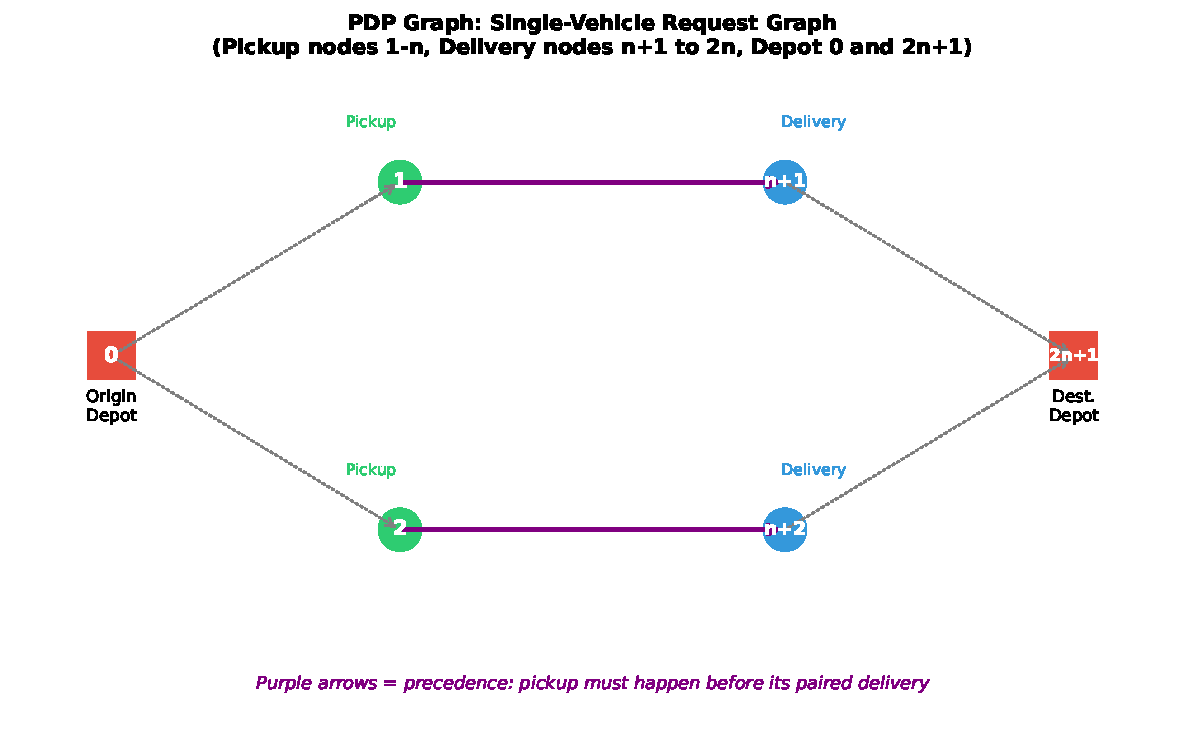
\includegraphics[width=0.72\textwidth]{fig_pdp_graph.pdf}
    \caption{The request graph for the PDPTW. Pickup nodes (green) are numbered $1 \ldots n$;
      delivery nodes (blue) are $n+1 \ldots 2n$; origin and destination depots are shown in red.
      Purple arrows indicate precedence: pickup $i$ must precede delivery $n+i$ on the same route.}
  \end{figure}

  \framebreak

  \begin{block}{PDPTW: Complete Integer Programme (Savelsbergh \& Sol, 1995)}
    \textbf{Decision variables:}
    \begin{itemize}
      \item $x_{ij}^k \in \{0,1\}$: equals 1 if vehicle $k$ travels directly from
            node $i$ to node $j$.
      \item $B_i^k \geq 0$: the time at which vehicle $k$ begins service at node $i$.
      \item $L_i^k \geq 0$: the load of vehicle $k$ when it departs node $i$.
    \end{itemize}

    \textbf{Objective -- minimise total travel cost:}
    \begin{equation}
      \min \sum_{k \in K} \sum_{i \in N} \sum_{j \in N} c_{ij} x_{ij}^k \tag{PDPTW-OBJ}
    \end{equation}

    \textbf{Constraints:}
    \begin{alignat}{2}
      \sum_{k \in K} \sum_{j \in N} x_{ij}^k &= 1
        &\quad& \forall i \in P \quad \text{(C1)}\\
      \sum_{j \in N} x_{0j}^k &= 1
        && \forall k \in K \quad \text{(C2)}\\
      \sum_{i \in N} x_{i,2n+1}^k &= 1
        && \forall k \in K \quad \text{(C3)}\\
      \sum_{j \in N} x_{ij}^k - \sum_{j \in N} x_{ji}^k &= 0
        && \forall i \in P \cup D,\ \forall k \quad \text{(C4)}\\
      \sum_{j \in N} x_{ij}^k &= \sum_{j \in N} x_{n+i,j}^k
        && \forall i \in P,\ \forall k \quad \text{(C5)}\\
      B_i^k + t_{ij} &\leq B_j^k + M(1-x_{ij}^k)
        && \forall i,j \in N,\ \forall k \quad \text{(C6)}\\
      B_i^k &\leq B_{n+i}^k
        && \forall i \in P,\ \forall k \quad \text{(C7)}\\
      e_i &\leq B_i^k \leq l_i
        && \forall i \in N,\ \forall k \quad \text{(C8)}\\
      L_j^k &\geq L_i^k + q_j x_{ij}^k - Q(1-x_{ij}^k)
        && \forall i,j \in N,\ \forall k \quad \text{(C9)}\\
      0 &\leq L_i^k \leq Q
        && \forall i \in N,\ \forall k \quad \text{(C10)}
    \end{alignat}
  \end{block}

  \framebreak

  \textbf{Symbol definitions in full:}

  \smallskip
  \begin{tabular}{@{}ll@{}}
    $K$ & set of vehicles (fleet) \\
    $P = \{1,\ldots,n\}$ & set of pickup nodes \\
    $D = \{n+1,\ldots,2n\}$ & set of delivery nodes \\
    $N = \{0\} \cup P \cup D \cup \{2n+1\}$ & complete node set including both depots \\
    $c_{ij}$ & cost of travelling from node $i$ to node $j$ \\
    $t_{ij}$ & travel time from node $i$ to node $j$ \\
    $[e_i, l_i]$ & time window at node $i$: earliest and latest service start \\
    $q_i$ & load change at $i$ ($+q_r$ at pickup, $-q_r$ at delivery) \\
    $Q$ & vehicle capacity \\
    $M$ & large constant (big-$M$ trick for logical implications) \\
    $B_i^k$ & time at which vehicle $k$ begins service at node $i$ \\
    $L_i^k$ & load of vehicle $k$ upon departure from node $i$ \\
  \end{tabular}

  \begin{figure}[h]
    \centering
    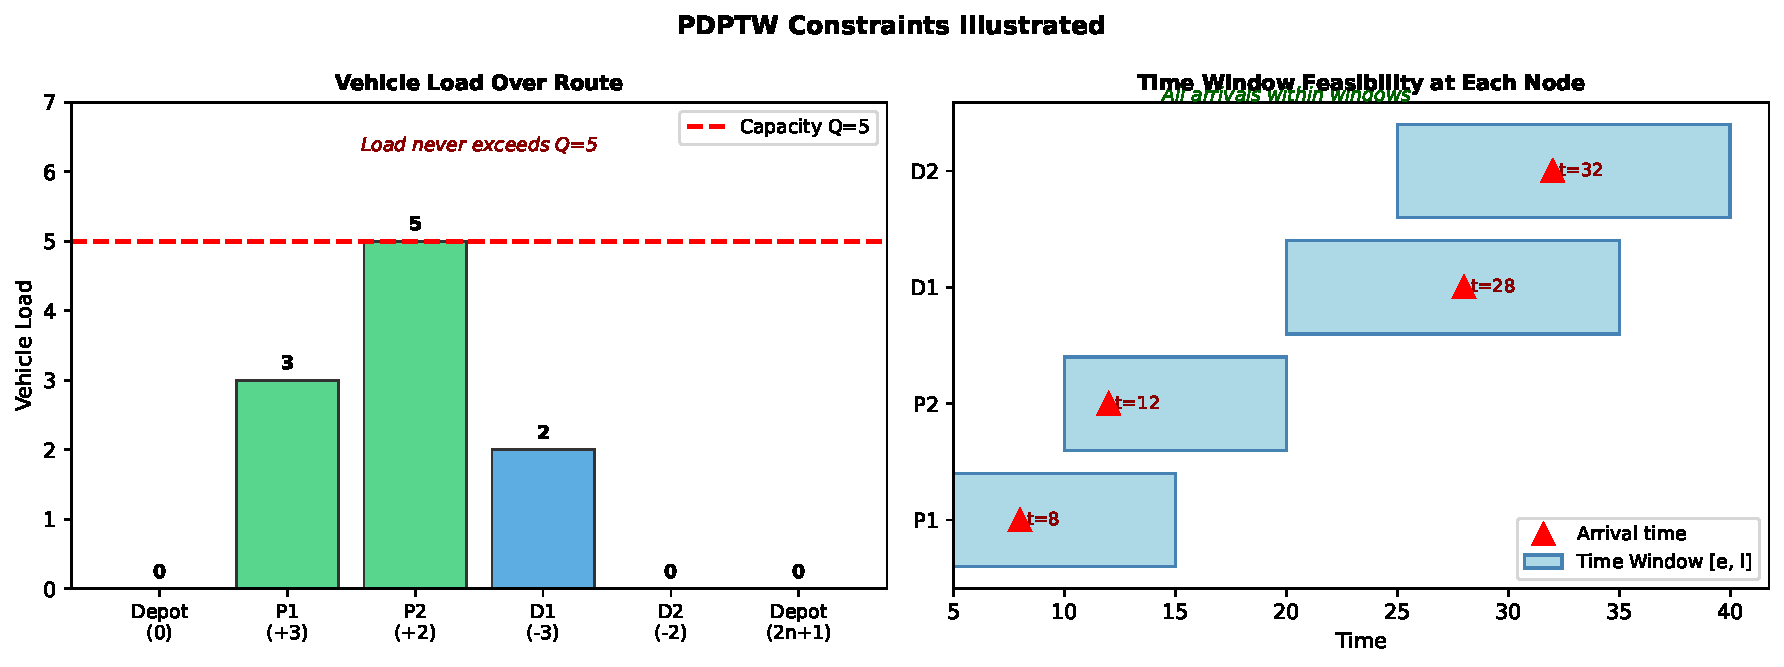
\includegraphics[width=0.82\textwidth]{fig_pdptw_constraints.pdf}
    \caption{Left: vehicle load along a 4-customer route; the horizontal dashed line marks
      capacity $Q=5$. Right: time windows (blue bars) and arrival times (red triangles)
      at each node. All arrivals fall within the specified windows, confirming feasibility.}
  \end{figure}

  \framebreak

  \textbf{Complexity.} The PDPTW is strongly NP-hard: it includes the Travelling Salesman
  Problem with time windows (TSPTW) as a special case, and even the single-vehicle version
  without time windows (PDTSP) is NP-hard.

  \textbf{Lower bound from LP relaxation.} Relaxing the integrality constraints
  ($x_{ij}^k \in [0,1]$) gives a linear programming relaxation. The LP bound is typically
  strengthened by adding valid inequalities:
  \begin{itemize}
    \item \textbf{Subtour elimination constraints} (SECs): prevent tours that do not
          include the depot.
    \item \textbf{Capacity-strengthening cuts}: based on minimum-cost flow subproblems.
    \item \textbf{Precedence-based cuts}: derived from the fact that pickup $i$ must
          precede delivery $n+i$ within any feasible route.
  \end{itemize}

  \begin{alertblock}{Key Insight: The 5 Key PDPTW Constraints}
    The PDPTW is harder than the VRPTW because of three additional constraints beyond
    capacity and time windows:
    (1) \textbf{Pairing:} pickup $i$ and delivery $n+i$ must be served by the same vehicle
    (constraint C5). (2) \textbf{Precedence:} pickup $i$ must precede delivery $n+i$
    (constraint C7). (3) \textbf{Route-based capacity:} the load must be feasible at every
    stop, not just in total (constraint C9--C10). These three constraints together make
    PDPTW significantly harder to decompose than the VRPTW.
  \end{alertblock}

\end{frame}

\begin{frame}[allowframebreaks]{6.4.2 Exact Methods for PDPTW}

  Exact methods for the PDPTW guarantee an optimal solution at the cost of potentially
  exponential running time. They are practical for instances up to roughly 50--75 requests
  depending on the tightness of the time windows.

  \textbf{Branch-and-cut (B\&C).}  The Branch-and-Cut method solves a sequence of LP
  relaxations strengthened by cutting planes, combined with a branch-and-bound tree search.
  The general scheme is:
  \begin{enumerate}
    \item \textbf{Solve LP relaxation} at the root node. If the optimal LP solution is
          integer, stop -- it is the optimal PDPTW solution. Otherwise, proceed.
    \item \textbf{Add cuts:} separate violated subtour elimination constraints, capacity
          cuts, and PDP-specific precedence cuts to tighten the LP relaxation.
    \item \textbf{Branch:} select a fractional variable $x_{ij}^k$ and create two
          sub-problems (branches): one fixing $x_{ij}^k = 0$ and one fixing $x_{ij}^k = 1$.
    \item \textbf{Prune:} if the LP lower bound of a node exceeds the incumbent upper
          bound, prune that branch.
    \item \textbf{Repeat} until all nodes are resolved.
  \end{enumerate}

  \begin{figure}[h]
    \centering
    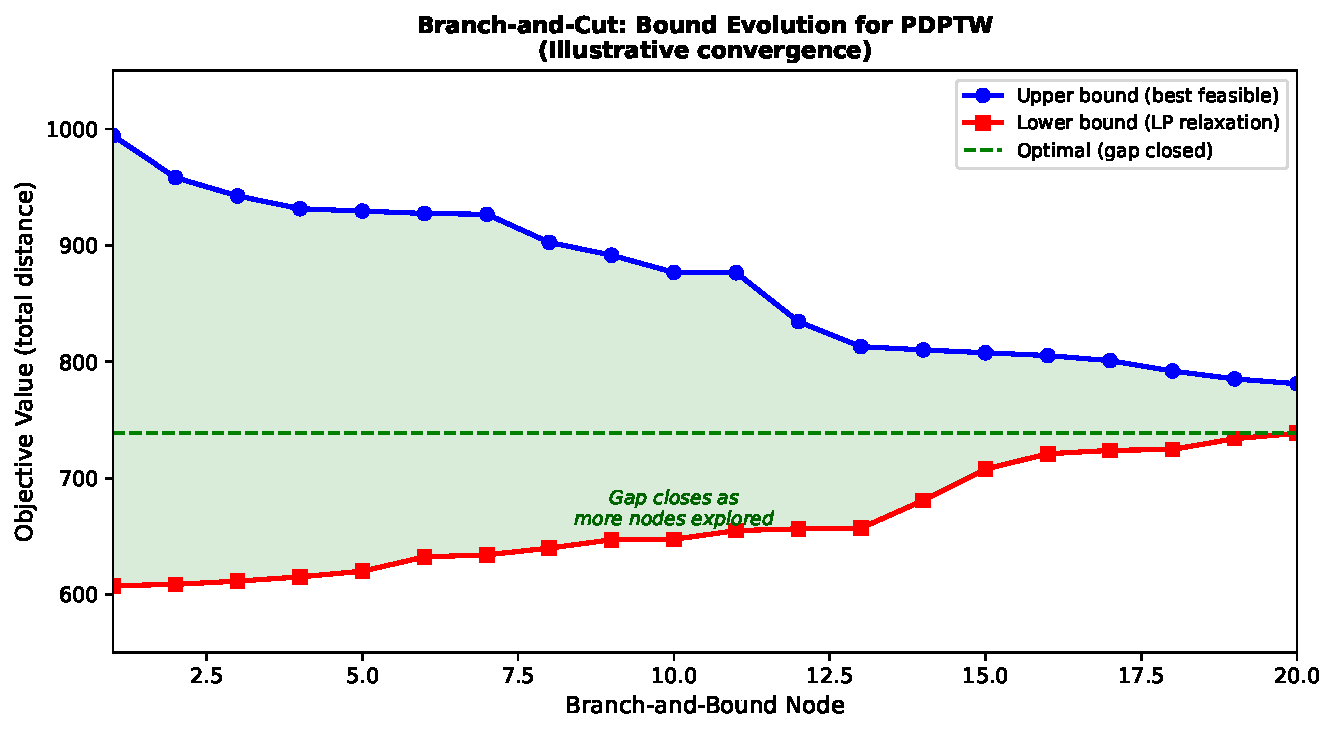
\includegraphics[width=0.55\textwidth]{fig_branch_cut.pdf}
    \caption{Illustrative convergence of the branch-and-cut method. The upper bound
      (best feasible solution found) decreases while the lower bound (LP relaxation)
      increases as more nodes are explored, until the gap is closed.}
  \end{figure}

  \framebreak

  \textbf{Key B\&C results for PDPTW.} Cordeau~(2006) proposed a branch-and-cut algorithm
  for the PDPTW that solved instances with up to 75 requests. The key ingredients were:
  \begin{itemize}
    \item \textbf{$k$-path inequalities:} violated if the current LP solution routes
          more than $k$ paths through a cut set, beyond what the capacity allows.
    \item \textbf{Clique-based lifted cover inequalities:} tighten capacity constraints
          by exploiting incompatibility between requests.
    \item \textbf{Branching on 3-cycles:} when many 3-cycle variables are fractional,
          branching on their indicator variables tends to close the LP gap quickly.
  \end{itemize}

  \textbf{Dynamic programming for single-vehicle PDPTW.}  When only one vehicle is
  available, the problem reduces to a sequencing problem. Exact DP formulations track the
  current time, current load, and the set of requests whose pickup has been made but
  delivery not yet completed (\emph{open requests}). The state space is exponential in the
  number of open requests, making DP practical only for small instances.

  \textbf{Column generation / Branch-and-Price.}  An alternative exact approach formulates
  the PDPTW as a \textbf{set-partitioning problem}:
  \[
    \min \sum_{r \in \Omega} c_r \lambda_r
    \quad \text{s.t.} \quad
    \sum_{r \in \Omega} a_{ir} \lambda_r = 1\ \forall i,\quad
    \lambda_r \in \{0,1\}
  \]
  where $\Omega$ is the set of all feasible routes, $c_r$ is the cost of route $r$, and
  $a_{ir} = 1$ if route $r$ serves request $i$.  Since $|\Omega|$ is exponentially large,
  column generation solves the LP relaxation by generating only routes with negative
  reduced cost -- the \textbf{pricing sub-problem} -- which is itself a shortest-path
  problem with resource constraints (SPPRC).

  \framebreak

  \textbf{Complexity summary for exact methods:}

  \begin{center}
    \begin{tabular}{lll}
      \toprule
      \textbf{Method}         & \textbf{Instance size} & \textbf{Key reference} \\
      \midrule
      Branch-and-cut          & $\leq 75$ requests      & Cordeau (2006) \\
      Branch-and-price        & $\leq 50$ requests      & Dumas et al. (1991) \\
      Dynamic programming     & $\leq 20$ requests      & Rais et al. (2014) \\
      \bottomrule
    \end{tabular}
  \end{center}

  \begin{alertblock}{Key Takeaway: Exact Methods}
    Branch-and-cut is the most powerful exact method for the PDPTW and can reliably
    solve instances with up to 75 requests. Beyond this scale, metaheuristics are
    necessary. The bottleneck for exact methods is the tightness of the LP bound: tight
    time windows dramatically reduce the search space and allow larger instances to be
    solved exactly.
  \end{alertblock}

\end{frame}

\begin{frame}[allowframebreaks]{6.4.3 Heuristics and Metaheuristics for PDPTW}

  Because the PDPTW is NP-hard, practical solvers rely on heuristics and metaheuristics
  that trade off solution quality for computational efficiency. The goal is to find
  near-optimal solutions quickly, especially for real-world instances with 100--1000 requests.

  \textbf{Construction heuristics.}  The most widely used construction approach for the
  PDPTW is the \textbf{parallel or sequential insertion heuristic}:
  \begin{enumerate}
    \item Start with $m$ routes, each containing only the depot.
    \item For each unassigned request, compute the \textbf{best feasible insertion} into
          every existing route -- the position that minimises the increase in total cost
          subject to precedence, capacity, and time-window constraints.
    \item Insert the request that can be cheaply inserted first (cheapest-first) or most
          urgently (most constrained first).
    \item Repeat until all requests are assigned.
  \end{enumerate}

  \begin{figure}[h]
    \centering
    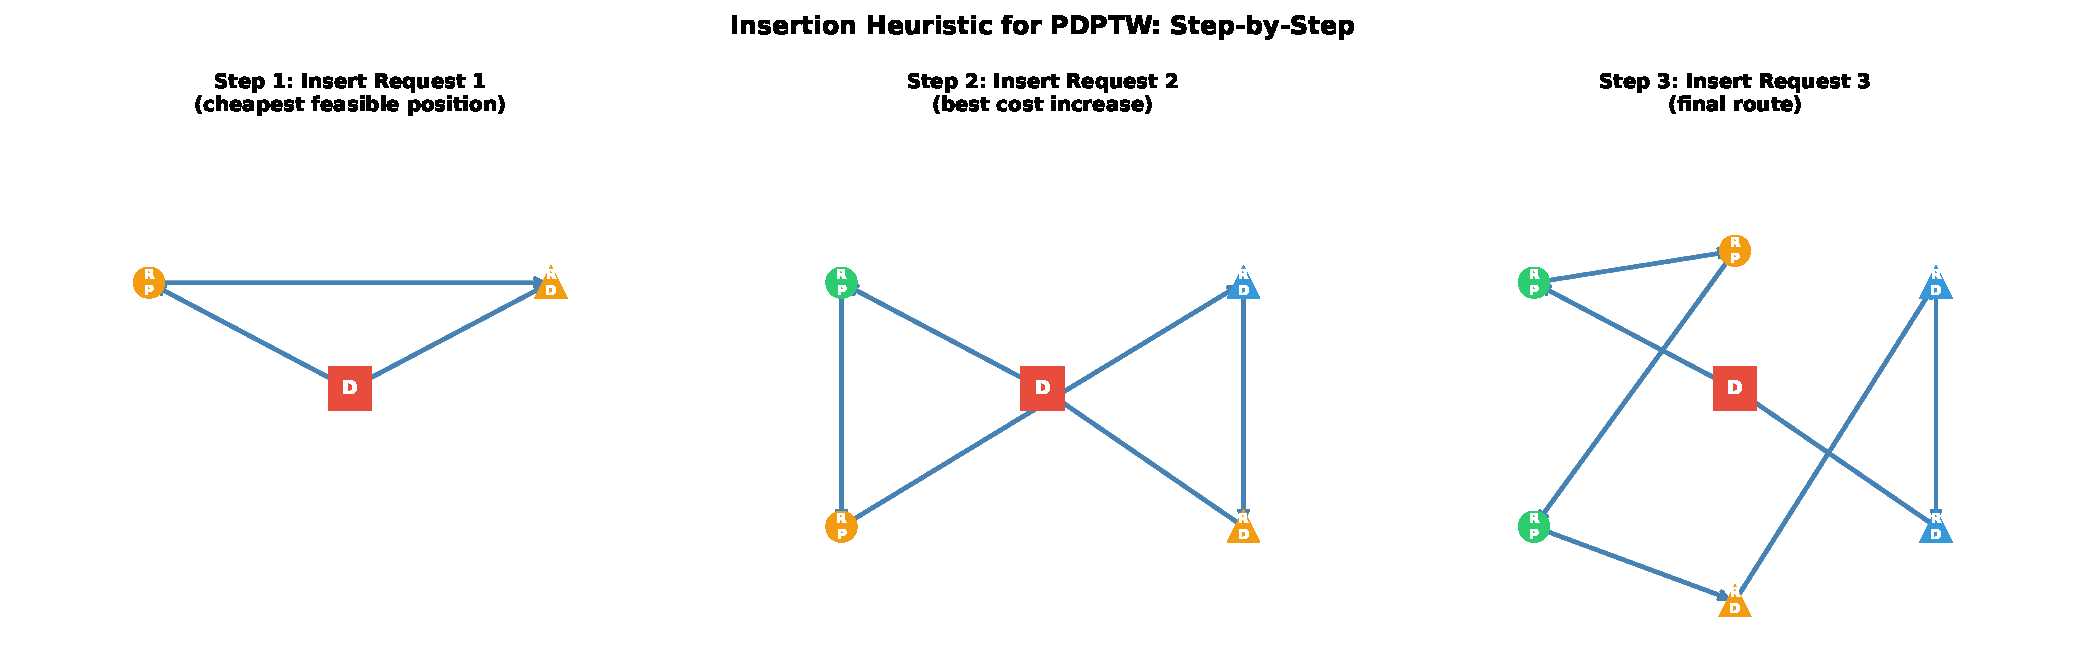
\includegraphics[width=0.88\textwidth]{fig_insertion_heuristic.pdf}
    \caption{Three-step insertion heuristic for a PDPTW with 3 requests. Step 1 inserts
      Request 1 (orange pair) to form the first partial route. Step 2 inserts Request 2
      at the best feasible position within the existing route. Step 3 inserts Request 3
      (orange) to produce the final solution.}
  \end{figure}

  \framebreak

  \textbf{Tabu Search (TS).}  Tabu Search was applied to the PDPTW by Nanry and Barnes
  (2000) and later extended by Li and Lim (2003), among others. The core idea is to
  explore the solution space by systematically making improving or, when no improvement
  exists, the least-worsening moves, while maintaining a \textbf{tabu list} of recently
  performed moves to avoid cycling.

  \begin{block}{Tabu Search Framework for PDPTW}
    \textbf{Input:} an initial feasible solution $s_0$; tabu tenure $T$; maximum
    iterations $I_{\max}$.\\
    \textbf{Output:} the best solution found $s^*$.
    \medskip

    \begin{enumerate}
      \item Set $s \leftarrow s_0$, $s^* \leftarrow s_0$, tabu list $\mathcal{T} \leftarrow \emptyset$.
      \item \textbf{For} $i = 1, 2, \ldots, I_{\max}$:
      \begin{enumerate}
        \item[a.] Generate the neighbourhood $\mathcal{N}(s)$ of $s$ by applying all
              feasible \emph{request-relocation} moves: remove a request $(p_i, d_{n+i})$
              from its current route and reinsert it at the best feasible position in
              the same or a different route.
        \item[b.] Select the best non-tabu move $m^*$ from $\mathcal{N}(s)$, or accept a
              tabu move if it satisfies the \textbf{aspiration criterion} (the resulting
              solution is better than $s^*$).
        \item[c.] Apply $m^*$: $s \leftarrow s \oplus m^*$.
        \item[d.] Add $m^*$ to $\mathcal{T}$; remove the oldest entry if $|\mathcal{T}| > T$.
        \item[e.] If $f(s) < f(s^*)$ then $s^* \leftarrow s$.
      \end{enumerate}
      \item Return $s^*$.
    \end{enumerate}
  \end{block}

  \framebreak

  \textbf{Neighbourhood structure for PDPTW TS.} The most effective neighbourhood for
  PDPTW TS uses \textbf{request relocation}: remove a (pickup, delivery) pair from its
  current route and reinsert it into another route (or the same route at a different
  position). The move must maintain feasibility -- precedence, capacity, and time windows.

  \begin{figure}[h]
    \centering
    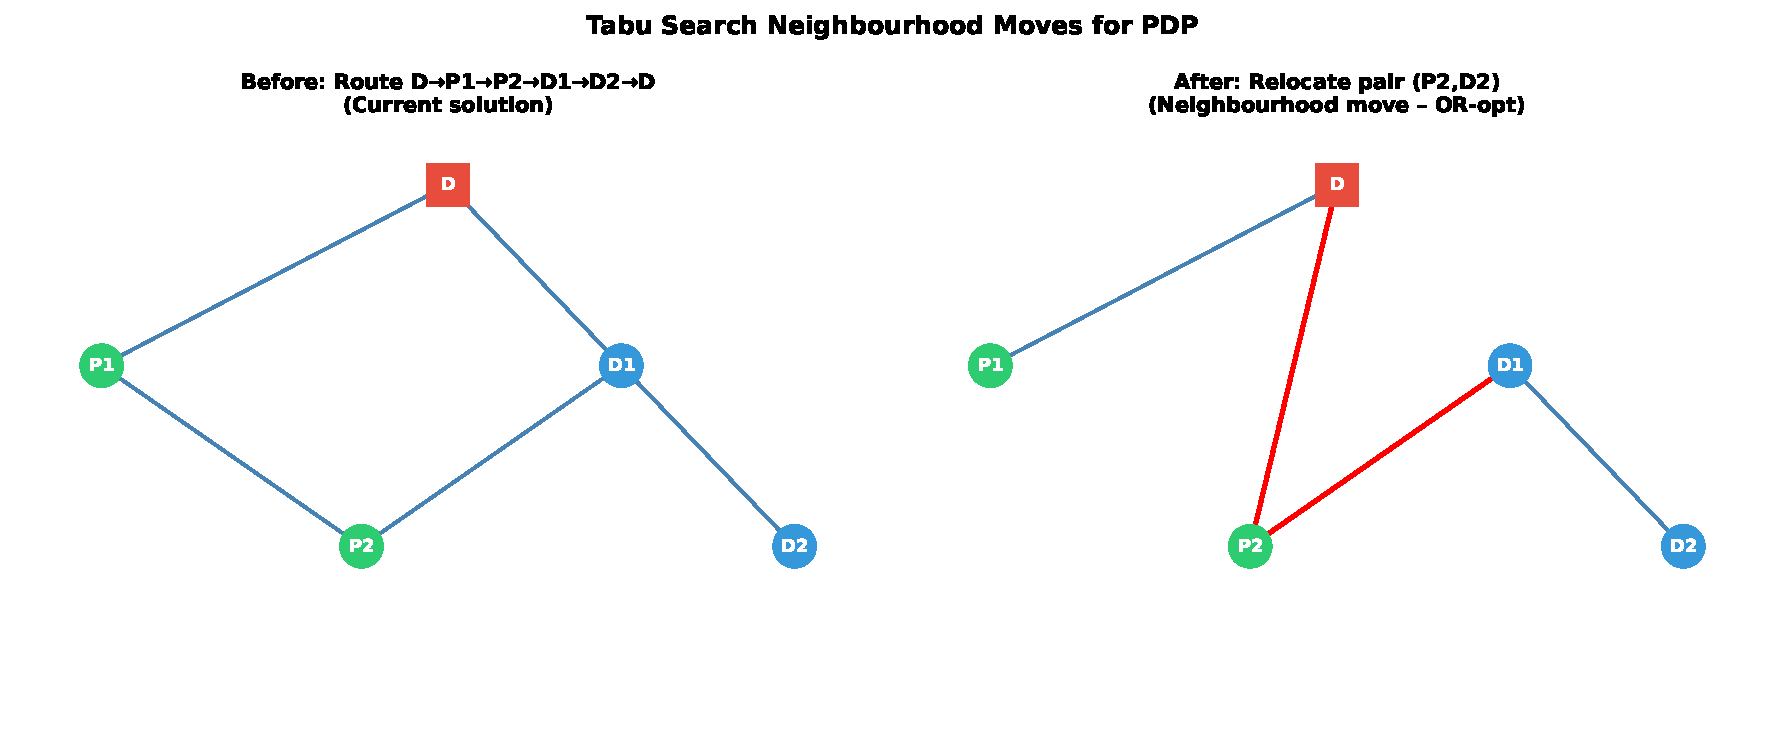
\includegraphics[width=0.60\textwidth]{fig_tabu_moves.pdf}
    \caption{Before and after a request-relocation neighbourhood move in PDPTW Tabu Search.
      The pair (P2, D2) is removed from route 1 and relocated to a different position
      (shown in red). After the move, both routes must remain feasible.}
  \end{figure}

  \textbf{Why does the tabu list help?} In local search without a tabu list, the algorithm
  tends to cycle between two solutions that are local optima of each other. The tabu list
  forbids reversing the most recent $T$ moves, forcing the search to explore new regions.
  Setting $T$ too small allows cycling; $T$ too large makes the search inflexible. Adaptive
  tabu tenures (randomly varying between $T_{\min}$ and $T_{\max}$) are common in practice.

  \framebreak

  \textbf{Large Neighbourhood Search (LNS) for PDPTW.} Ropke and Pisinger (2006) proposed
  LNS as an effective method for the PDPTW. The algorithm iteratively:
  \begin{enumerate}
    \item \textbf{Destroys} part of the current solution by removing $q$ requests
          (where $q$ is a \emph{destroy degree}, typically $q \approx 0.1 \cdot n$ to
          $0.4 \cdot n$).
    \item \textbf{Repairs} the partial solution by reinserting the removed requests using
          a greedy insertion heuristic.
    \item \textbf{Accepts} the new solution according to a simulated annealing criterion:
          $s_{\text{new}}$ is accepted if $f(s_{\text{new}}) < f(s)$, or with probability
          $\exp(-(f(s_{\text{new}}) - f(s)) / T)$ if $f(s_{\text{new}}) \geq f(s)$.
  \end{enumerate}

  \begin{block}{LNS Destroy Operators}
    \begin{itemize}
      \item \textbf{Random removal:} select $q$ requests uniformly at random.
      \item \textbf{Shaw removal:} remove $q$ requests that are \emph{similar} to each
            other, where similarity is measured by geographic proximity and time-window
            overlap. The idea is that similar requests are easier to mutually reassign.
      \item \textbf{Worst removal:} remove the $q$ requests with the highest contribution
            to the total solution cost (the most expensive requests).
    \end{itemize}
  \end{block}

  \framebreak

  \textbf{Adaptive LNS (ALNS).} Ropke and Pisinger (2006) extended LNS to the
  \textbf{Adaptive Large Neighbourhood Search (ALNS)} by maintaining a \emph{pool} of
  destroy and repair operators, and dynamically adjusting the probability of selecting
  each operator based on its historical performance:

  \begin{itemize}
    \item Each operator $o$ is assigned a score $\pi_o$ that accumulates reward whenever
          the operator contributes to a new best solution, an improving solution, or an
          accepted non-improving solution.
    \item After every $\sigma$ iterations (a \emph{segment}), the selection probability of
          each operator is updated:
          \[
            p_o \leftarrow \frac{w_o}{\sum_{o'} w_{o'}}, \quad
            w_o \leftarrow (1-r) w_o + r \frac{\pi_o}{\theta_o}
          \]
          where $w_o$ is the weight, $r \in (0,1)$ is a reaction factor controlling how
          quickly weights adapt, and $\theta_o$ is the number of times operator $o$ was
          used during the segment.
    \item Operators that consistently find better solutions receive higher probability
          of being selected in subsequent iterations.
  \end{itemize}

  \textbf{Why ALNS works.} Different destroy operators are effective for different types
  of problem structure. Random removal provides diversification; Shaw removal provides
  intensification around related requests; worst removal targets high-cost areas.
  Adapting probabilities ensures the algorithm exploits whichever strategy is most
  effective for the current instance.

  \framebreak

  \begin{exampleblock}{ALNS Numerical Illustration: Score Update}
    Suppose the algorithm has 3 destroy operators: Random (R), Shaw (S), Worst (W).
    After one segment of $\sigma=50$ iterations, the collected statistics are:
    \begin{center}
      \begin{tabular}{lcccc}
        \toprule
        \textbf{Operator} & $\theta_o$ (uses) & $\pi_o$ (score) & $w_o$ (old) & $w_o$ (new, $r=0.2$) \\
        \midrule
        Random (R) & 18 & 24 & 1.00 & $0.8 \times 1.00 + 0.2 \times (24/18) = 1.067$ \\
        Shaw (S)   & 17 & 38 & 1.00 & $0.8 \times 1.00 + 0.2 \times (38/17) = 1.247$ \\
        Worst (W)  & 15 & 12 & 1.00 & $0.8 \times 1.00 + 0.2 \times (12/15) = 0.960$ \\
        \bottomrule
      \end{tabular}
    \end{center}
    The selection probabilities become: $p_R = 1.067/3.274 = 0.326$;
    $p_S = 1.247/3.274 = 0.381$; $p_W = 0.960/3.274 = 0.293$. Shaw removal, having
    found the most improvements, now has the highest selection probability.
  \end{exampleblock}

  \framebreak

  \textbf{Branch-and-Cut integrated with heuristics.} Ropke et al.~(2007) combined
  branch-and-cut with LNS in a so-called \textbf{matheuristic} framework: the LNS is
  used to find a good upper bound, which is then passed to the B\&C as the incumbent,
  greatly reducing the B\&C search tree.

  \textbf{POPMUSIC.} For very large PDPTW instances (several hundred requests), the
  POPMUSIC framework (Partial Optimisation Metaheuristic Under Special Intensification
  Conditions) by Taillard et al.\ has been adapted: the problem is decomposed into
  overlapping sub-problems of manageable size, each sub-problem is optimised by a
  fast metaheuristic, and the solutions are stitched back together.

  \begin{figure}[h]
    \centering
    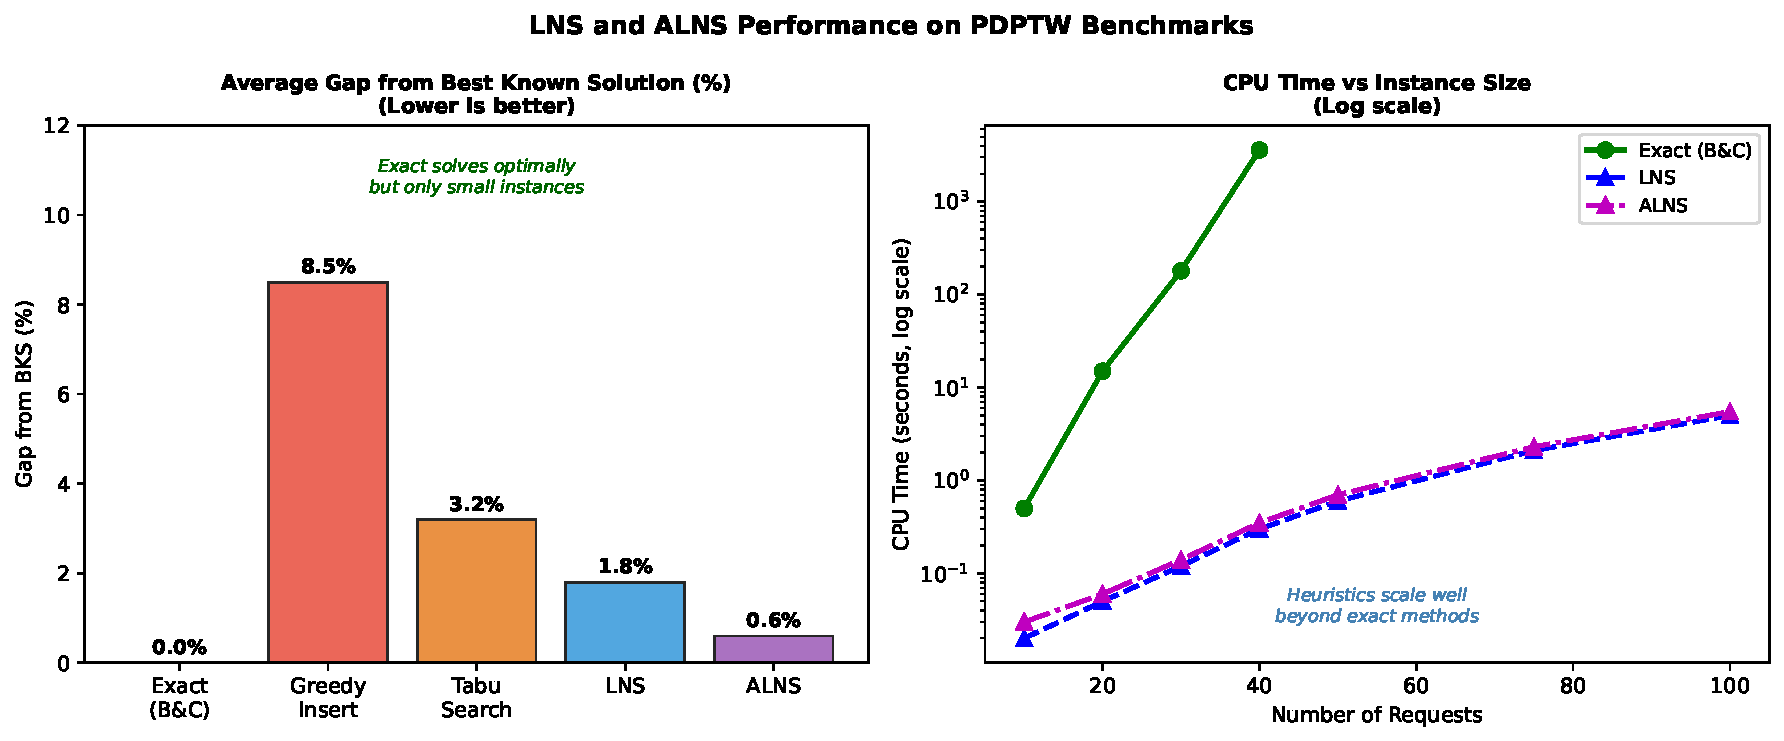
\includegraphics[width=0.80\textwidth]{fig_lns_performance.pdf}
    \caption{Left: average gap from best known solution for different methods on PDPTW
      benchmarks. ALNS achieves solutions within 0.6\% of BKS. Right: CPU time vs instance
      size (log scale); exact B\&C is practical only for small instances while LNS and ALNS
      scale to hundreds of requests.}
  \end{figure}

  \begin{alertblock}{Key Takeaway: Metaheuristics for PDPTW}
    ALNS is currently the leading metaheuristic for the PDPTW, offering the best
    balance of solution quality and scalability. The key design choice is the set of
    destroy/repair operators: combining random, similarity-based (Shaw), and worst-case
    removal with adaptive operator selection has proven highly effective across diverse
    benchmark sets.
  \end{alertblock}

\end{frame}

\begin{frame}[allowframebreaks]{6.4.4 Single-Vehicle PDPTW}

  When the fleet consists of a single vehicle, the PDPTW reduces to the
  \textbf{Pickup-and-Delivery TSP with Time Windows (PDTSPTW)}.  This problem has been
  studied both as a theoretical object and as a sub-problem in column generation approaches
  to the multi-vehicle PDPTW.

  \textbf{Single-vehicle exact algorithm.} Ruland and Rodin~(1997) proposed a branch-and-cut
  algorithm specifically for the single-vehicle case.  The key observation is that for a
  single vehicle, the constraint that the same vehicle serves both endpoints of each request
  is automatically satisfied.  The remaining difficulty is the combination of:
  \begin{itemize}
    \item Precedence constraints: pickup $i$ before delivery $n+i$.
    \item Capacity constraints: load $\in [0, Q]$ throughout.
    \item Time window constraints: service within $[e_i, l_i]$ at each node.
  \end{itemize}

  \textbf{Algorithms for the single-vehicle PDTSP (no time windows).} Without time windows,
  the problem simplifies to the PDTSP. Hernandez-Perez and Salazar-Gonzalez proposed a
  branch-and-cut that uses a clever reformulation: they observe that the PDTSP is
  equivalent to the TSP on a reduced graph where infeasible arcs (those that would violate
  precedence or capacity) are removed. Their algorithm solves instances with up to 40 nodes.

  \begin{alertblock}{Key Takeaway: Single-Vehicle PDPTW}
    The single-vehicle PDPTW is important as a sub-problem in column generation for
    the multi-vehicle case. Efficient algorithms for it (particularly those that generate
    optimal routes quickly) are critical to the scalability of branch-and-price methods
    for the full multi-vehicle PDPTW.
  \end{alertblock}

\end{frame}

\begin{frame}[allowframebreaks]{6.4.5 Multiple-Vehicle PDPTW}

  In the multi-vehicle setting, a fleet $K$ of identical vehicles must collectively serve
  all $n$ requests. This is the standard industrial setting and the most studied variant
  in the literature.

  \begin{figure}[h]
    \centering
    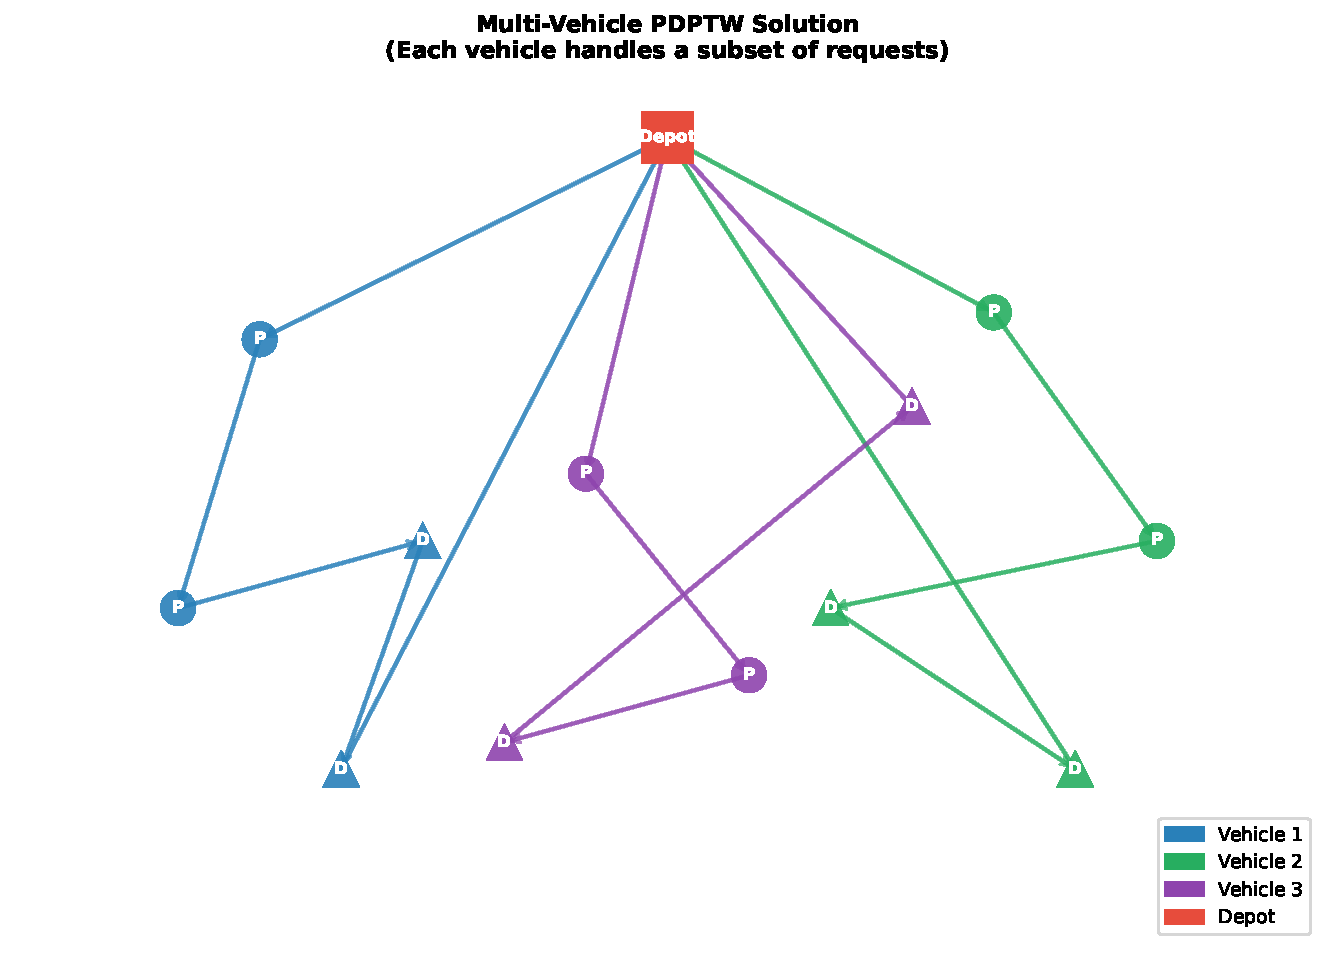
\includegraphics[width=0.65\textwidth]{fig_multiple_vehicles.pdf}
    \caption{A multi-vehicle PDPTW solution with 3 vehicles (blue, green, purple). Each
      vehicle serves a subset of pickup-delivery pairs. All routes start and end at the
      depot. Triangles denote delivery nodes; circles denote pickup nodes.}
  \end{figure}

  \textbf{LKH (Lin-Kernighan-Helsgott) heuristics.} Several authors have adapted the
  powerful LKH algorithm (originally for the TSP) to the PDPTW. The key challenge is
  incorporating the pairing and precedence constraints into the LKH-style edge exchange
  moves. The most successful adaptations maintain feasibility at every step by rejecting
  moves that violate precedence or capacity.

  \framebreak

  \textbf{Population-based methods.} Genetic algorithms and evolutionary approaches have
  also been applied to the multi-vehicle PDPTW:
  \begin{itemize}
    \item \textbf{Representation:} a chromosome encodes the sequence of requests assigned
          to each vehicle, with the constraint that for each vehicle's sub-sequence, the
          pickup of request $i$ must appear before the delivery.
    \item \textbf{Crossover operators:} order-based crossover (OBX) and position-based
          crossover (PBX) are adapted to maintain precedence feasibility.
    \item \textbf{Mutation operators:} relocation of a (pickup, delivery) pair within
          the same route or between routes.
    \item \textbf{Fitness:} total travel cost plus a penalty for constraint violations.
  \end{itemize}

  \textbf{Benchmark instances.} The standard benchmarks for the multi-vehicle PDPTW are
  due to Li and Lim~(2003), who proposed 12 instance categories (n100--n1000) with
  varying time window tightness and vehicle capacity. These have been solved to near-optimal
  by several metaheuristics including ALNS (Ropke \& Pisinger, 2006) and its variants.

  \textbf{Correlation with VRPTW.} When all pickups are at the depot and all deliveries
  are at customers, the PDPTW reduces to the VRPTW. This means that any lower bound or
  algorithm for the VRPTW can be adapted for the PDPTW, though the additional constraints
  make the PDPTW typically harder.

  \begin{alertblock}{Key Takeaway: Multi-Vehicle PDPTW}
    The multi-vehicle PDPTW is the canonical problem in goods PDP. ALNS by Ropke and
    Pisinger (2006) remains the state-of-the-art metaheuristic, closing the gap to
    known optima to within 1\% on Li-Lim benchmark instances up to 100 requests.
    For exact methods, branch-and-cut handles up to 75 requests; column generation
    extends this range somewhat but remains impractical for large instances.
  \end{alertblock}

\end{frame}

% ── Python implementation ─────────────────────────────────
\begin{frame}[fragile]{Python: PDPTW Feasibility Check and Greedy Construction}
\begin{lstlisting}
"""
PDPTW feasibility checker and greedy insertion heuristic.
Assumes symmetric travel cost/time: dist[i][j] == dist[j][i].
"""
from dataclasses import dataclass, field
from typing import List, Tuple, Optional
import math

@dataclass
class Request:
    idx: int           # request id (1..n)
    pickup: int        # pickup node index
    delivery: int      # delivery node index
    load: float        # goods quantity
    e_p: float         # earliest service at pickup
    l_p: float         # latest service at pickup
    e_d: float         # earliest service at delivery
    l_d: float         # latest service at delivery

def is_feasible(route: List[int], requests: dict, dist: List[List[float]],
                capacity: float, service_time: float = 0.0) -> bool:
    """
    Check if a route is feasible for PDPTW.
    route: list of node indices including depot (0) at start and end.
    requests: dict mapping pickup_node -> Request object.
    Returns True if precedence, capacity, and time windows are all satisfied.
    """
    n = max(r.delivery for r in requests.values())
    # Build time windows and loads indexed by node
    tw = {}; load_delta = {}
    for req in requests.values():
        tw[req.pickup]   = (req.e_p, req.l_p)
        tw[req.delivery] = (req.e_d, req.l_d)
        load_delta[req.pickup]   = +req.load
        load_delta[req.delivery] = -req.load
    tw[0] = (0, math.inf)  # depot: no time restriction

    # Check precedence: for each request, pickup must appear before delivery
    for req in requests.values():
        p_pos = route.index(req.pickup) if req.pickup in route else -1
        d_pos = route.index(req.delivery) if req.delivery in route else -1
        if p_pos == -1 or d_pos == -1:
            return False  # both endpoints must be in route
        if p_pos >= d_pos:
            return False  # pickup must strictly precede delivery

    # Check capacity and time windows along route
    load = 0.0; time = 0.0
    for k in range(len(route)):
        node = route[k]
        if k > 0:
            time += dist[route[k-1]][node]
        e, l = tw.get(node, (0, math.inf))
        time = max(time, e)  # wait if arriving early
        if time > l:
            return False  # time window violated
        time += service_time
        load += load_delta.get(node, 0)
        if load < 0 or load > capacity:
            return False  # capacity violated
    return True

def greedy_insert_pdptw(requests: List[Request], dist: List[List[float]],
                         capacity: float) -> List[List[int]]:
    """
    Sequential greedy insertion for PDPTW.
    Returns a list of routes (each route is a list of node indices).
    """
    routes = [[0, 0]]  # start with one route: depot -> depot
    unassigned = list(requests)

    while unassigned:
        best_cost = math.inf
        best_req = None; best_route_idx = None; best_positions = None

        for req in unassigned:
            for r_idx, route in enumerate(routes):
                # Try all feasible positions for pickup and delivery
                n = len(route)
                for p_pos in range(1, n):
                    for d_pos in range(p_pos + 1, n + 1):
                        new_route = (route[:p_pos] + [req.pickup] +
                                     route[p_pos:d_pos] + [req.delivery] +
                                     route[d_pos:])
                        req_dict = {r.pickup: r for r in requests}
                        if is_feasible(new_route, req_dict, dist, capacity):
                            old_cost = sum(dist[route[i]][route[i+1]]
                                           for i in range(len(route)-1))
                            new_cost = sum(dist[new_route[i]][new_route[i+1]]
                                           for i in range(len(new_route)-1))
                            delta = new_cost - old_cost
                            if delta < best_cost:
                                best_cost = delta
                                best_req = req
                                best_route_idx = r_idx
                                best_positions = (p_pos, d_pos)

        if best_req is None:
            # No feasible insertion in existing routes: open a new route
            routes.append([0, best_req.pickup, best_req.delivery, 0]
                          if best_req else [0, 0])
            unassigned.pop(0)
        else:
            p_pos, d_pos = best_positions
            route = routes[best_route_idx]
            routes[best_route_idx] = (route[:p_pos] + [best_req.pickup] +
                                       route[p_pos:d_pos] + [best_req.delivery] +
                                       route[d_pos:])
            unassigned.remove(best_req)

    return routes
\end{lstlisting}
\end{frame}

% ============================================================
\section{Problems with Loading Constraints}
% ============================================================

\begin{frame}[allowframebreaks]{6.5 Problems with Loading Constraints}

  In practice, goods transported by vehicles are physical three-dimensional objects.
  The order in which goods are loaded onto a vehicle determines whether they can be
  unloaded at each delivery stop without disturbing other cargo. This gives rise to
  \textbf{loading-constrained PDPs} -- problems in which both the routing and the
  loading plan must be co-optimised.

  \begin{figure}[h]
    \centering
    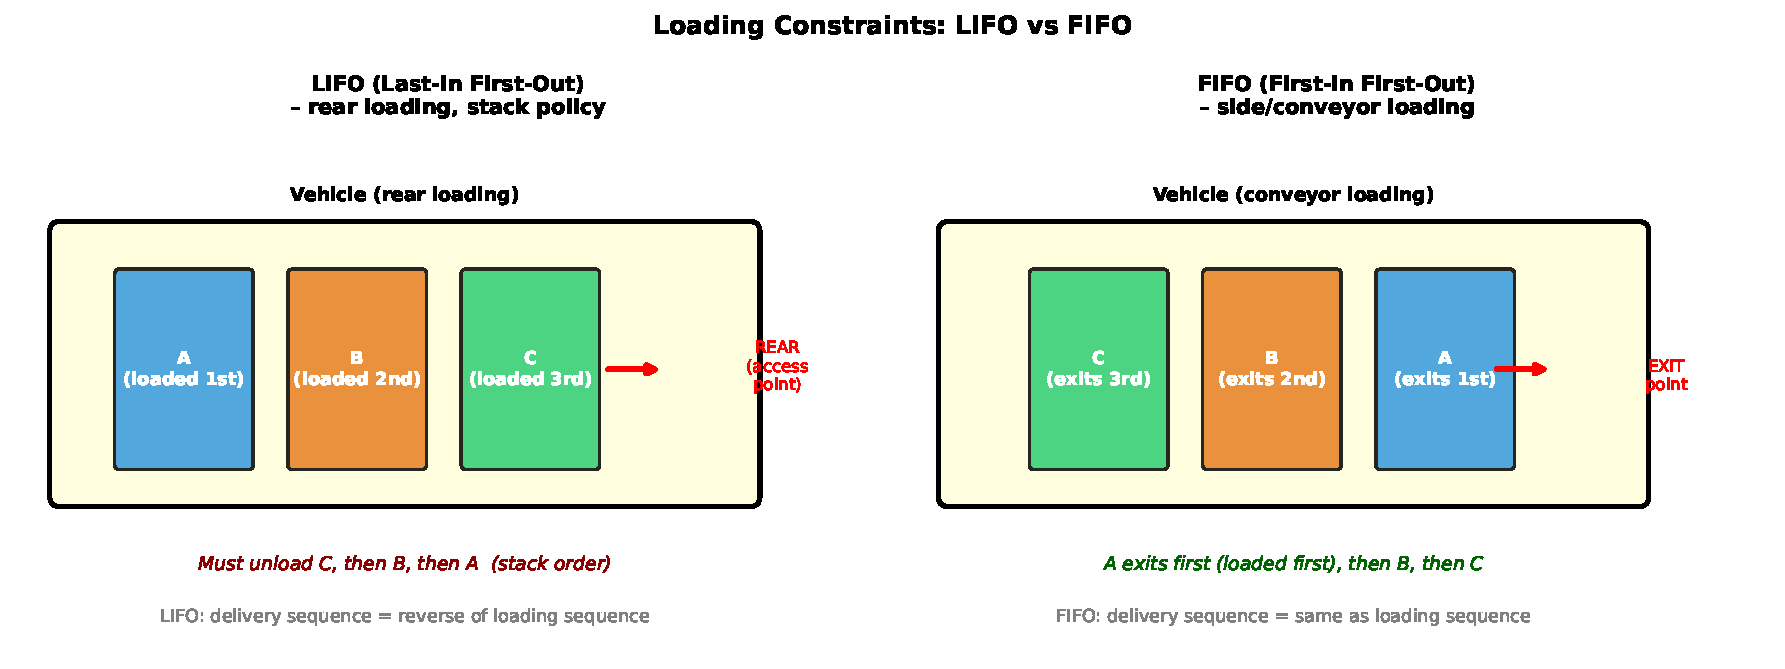
\includegraphics[width=0.85\textwidth]{fig_loading_constraints.pdf}
    \caption{Left: LIFO loading -- items loaded first (deepest inside the vehicle) must
      be delivered last; items near the rear are delivered first. Right: FIFO loading --
      items loaded first exit first (conveyor-style). The delivery sequence on the route
      must respect the physical loading order.}
  \end{figure}

  \framebreak

  \textbf{Three types of loading constraints:}
  \begin{enumerate}
    \item \textbf{LIFO (Last-In First-Out):} the vehicle is accessed from the rear only
          (like a stack). The most recently loaded item must be unloaded first. This means
          the \emph{delivery sequence must be the reverse of the loading sequence}: if item
          $A$ is loaded before item $B$, then $B$ must be delivered before $A$.
    \item \textbf{FIFO (First-In First-Out):} the vehicle is a conveyor -- items loaded
          first exit first. The delivery sequence must \emph{match} the loading sequence.
    \item \textbf{3D Loading:} items have explicit three-dimensional extents (length,
          width, height) and must physically fit inside the container at every stage of
          the route. This requires solving a bin-packing sub-problem at each delivery stop.
  \end{enumerate}

  \begin{block}{LIFO Constraint: Formal Statement}
    Let $\sigma$ be the route sequence of customers visited by a vehicle, and let
    $\pi$ be the loading order (order in which items are placed onto the vehicle).
    The LIFO constraint states:

    \textbf{For any two items $i$ and $j$ carried by the same vehicle, if $i$ is
    delivered before $j$ (i.e., $i$ comes before $j$ in the route), then $j$ must
    have been loaded before $i$ (i.e., $j$ precedes $i$ in the loading order).}

    Equivalently: $\text{position}(\text{deliver}\ i) < \text{position}(\text{deliver}\ j)
    \Rightarrow \text{position}(\text{load}\ j) < \text{position}(\text{load}\ i)$.
  \end{block}

  \framebreak

  \textbf{PDPTW with LIFO constraints.} Carrabs, Cordeau, and Laporte~(2007) studied the
  \textbf{PDPTW-L} (PDPTW with LIFO constraints) and showed that:
  \begin{itemize}
    \item LIFO constraints can be enforced without explicitly tracking the loading order:
          it suffices to check that the route does not contain any \emph{interleaving} pair.
          Two requests $i$ and $j$ are \textbf{interleaved} if the route visits them in
          the order $p_i, p_j, d_i, d_j$ (or $p_j, p_i, d_j, d_i$). LIFO feasibility
          requires that no such interleaving occurs.
    \item Equivalently: for every pair of requests on the same vehicle, the pickup-delivery
          intervals must be either \emph{nested} (one contained within the other) or
          \emph{disjoint} (non-overlapping).
  \end{itemize}

  \begin{exampleblock}{LIFO Interleaving: Worked Example}
    Suppose a route visits nodes in order: $\text{Depot}, P_1, P_2, D_1, D_2, \text{Depot}$.
    \begin{itemize}
      \item Requests: $(P_1, D_1)$ and $(P_2, D_2)$.
      \item Position of $P_1 = 1$, $P_2 = 2$, $D_1 = 3$, $D_2 = 4$.
      \item The sequence $P_1 < P_2 < D_1 < D_2$ means the intervals $[1,3]$ and $[2,4]$
            \emph{overlap but neither is contained in the other} -- this is \textbf{interleaved}.
      \item A LIFO-feasible alternative: $\text{Depot}, P_1, P_2, D_2, D_1, \text{Depot}$
            gives intervals $[1,4]$ and $[2,3]$ -- interval $[2,3]$ is \textbf{nested}
            inside $[1,4]$. This satisfies LIFO: item 2 (loaded after item 1 at $P_2$)
            is delivered first at $D_2$, then item 1 at $D_1$. \checkmark
    \end{itemize}
  \end{exampleblock}

  \framebreak

  \textbf{Algorithms for PDPTW-L.} Carrabs et al.\ (2007) designed a Branch-and-Cut
  algorithm for PDPTW-L that incorporates specific valid inequalities for LIFO feasibility.
  The branch-and-cut was able to solve instances with up to 25 requests.

  For larger instances, heuristic approaches are necessary:
  \begin{itemize}
    \item \textbf{Tabu Search:} the neighbourhood moves must be restricted to those that
          maintain LIFO feasibility. A swap move that creates an interleaving is rejected.
    \item \textbf{LNS with LIFO repair:} after removing a subset of requests, the repair
          heuristic inserts them at positions that maintain the nesting property.
    \item \textbf{Dynamic programming:} for a single vehicle, DP can track the set of
          currently open (picked up but not yet delivered) requests and ensure LIFO ordering
          at each step.
  \end{itemize}

  \textbf{PDPTW with FIFO constraints.} The PDPTW-F (FIFO variant) has analogous
  structure: instead of nesting, the pickup-delivery intervals must be \emph{compatible}
  in the FIFO sense. Ladier and Alpan~(2016) and others have shown that FIFO constraints
  arise naturally in conveyor-loading contexts such as airport baggage handling.

  \framebreak

  \textbf{3D Loading PDP.}  The most complex loading variant requires that items be
  physically packed into the vehicle's container in three dimensions.  At every delivery
  stop, the item to be unloaded must be accessible from the door without requiring other
  items to be moved.

  \begin{figure}[h]
    \centering
    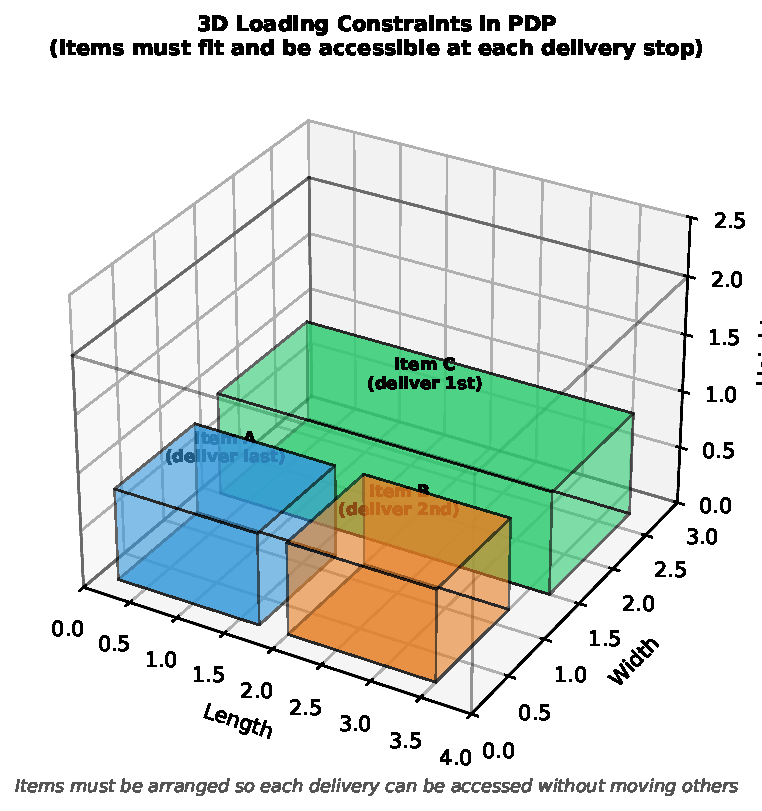
\includegraphics[width=0.62\textwidth]{fig_3d_loading.pdf}
    \caption{3D loading constraint illustration. Item C (to be delivered first) is placed
      near the door. Items A and B are stacked behind it. The physical dimensions (length,
      width, height) of all items must be accounted for to ensure stability and accessibility.}
  \end{figure}

  \textbf{The 3L-PDPTW (Three-dimensional Loading PDPTW).}  In this variant, each
  request is a set of rectangular boxes with specified dimensions. The constraints are:
  \begin{enumerate}
    \item \textbf{Routing:} standard PDPTW constraints (precedence, capacity, time windows).
    \item \textbf{Packing:} at each point in the route, the boxes on board must physically
          fit inside the vehicle container, satisfying non-overlap and stability constraints.
    \item \textbf{Sequential accessibility:} when the vehicle arrives at delivery $i$,
          the boxes for request $i$ must be reachable from the loading door without
          removing boxes intended for later deliveries.
  \end{enumerate}

  The coupling between routing and packing makes this problem substantially harder than
  either PDPTW or 3D bin-packing alone. Metaheuristics for the 3L-PDPTW typically use
  a \textbf{two-level approach}: the outer level optimises the route using LNS or Tabu
  Search, and the inner level calls a heuristic packing algorithm (e.g., a greedy
  best-fit decreasing algorithm) to check feasibility of any candidate route.

  \begin{alertblock}{Key Takeaway: Loading-Constrained PDPs}
    Loading constraints (LIFO, FIFO, 3D) fundamentally couple the loading plan with
    the route sequence, making the problem harder than standard PDPTW. LIFO constraints
    can be enforced by forbidding interleaved request intervals (no interleaving condition).
    3D loading requires a co-optimisation of routing and bin-packing and is best
    handled by two-level metaheuristics.
  \end{alertblock}

\end{frame}

\begin{frame}[allowframebreaks]{6.5.1 One-to-One Problems with Loading Constraints}

  The one-to-one structure is the most natural setting for loading-constrained PDPs,
  since each request has a dedicated item to be picked up and delivered. Research has
  focused on two specific settings:

  \textbf{Single-vehicle PDPTW with LIFO.}  Carrabs, Cordeau, and Laporte~(2007)
  proposed a Branch-and-Cut based on the following key result: LIFO feasibility of a
  route can be verified in $O(n)$ time by scanning the route and maintaining a stack.
  If, when attempting to deliver item $i$, the top of the stack is not $i$, the route
  is LIFO-infeasible.

  \textbf{Algorithm (LIFO Feasibility Check):}
  \begin{enumerate}
    \item Initialise an empty stack $S$.
    \item Scan the route from the depot to the end:
      \begin{itemize}
        \item If the current node is a \textbf{pickup} $p_i$: push $i$ onto $S$.
        \item If the current node is a \textbf{delivery} $d_i$: if $\text{top}(S) = i$,
              pop $S$; else the route is \textbf{LIFO-infeasible}.
      \end{itemize}
    \item If the stack is empty at the end, the route is LIFO-feasible.
  \end{enumerate}

  \begin{exampleblock}{LIFO Stack Check: Example}
    Route: $\text{Depot}, P_1, P_3, D_3, P_2, D_2, D_1, \text{Depot}$.
    \begin{center}
      \begin{tabular}{lcl}
        \toprule
        \textbf{Node} & \textbf{Action} & \textbf{Stack} \\
        \midrule
        $P_1$ & Push 1 & $\{1\}$ \\
        $P_3$ & Push 3 & $\{1, 3\}$ \\
        $D_3$ & Top = 3, Pop & $\{1\}$ \\
        $P_2$ & Push 2 & $\{1, 2\}$ \\
        $D_2$ & Top = 2, Pop & $\{1\}$ \\
        $D_1$ & Top = 1, Pop & $\{\}$ \\
        \bottomrule
      \end{tabular}
    \end{center}
    Stack empty at end: route is \textbf{LIFO-feasible}. \checkmark
    The structure shows nested intervals: $[P_1,D_1]$ contains $[P_2,D_2]$, which
    is disjoint from $[P_3,D_3]$.
  \end{exampleblock}

  \framebreak

  \textbf{One-to-Many-to-One with Loading Constraints.}  In the 1-M-1 setting,
  Salazar-Gonzalez~(2014) considered a variant where the same vehicle delivers goods
  from the depot (forward logistics) and collects returned goods (reverse logistics) on
  the same tour. LIFO constraints arise because the vehicle is loaded at the depot in a
  specific order that constrains the delivery sequence.

  \textbf{Incorporating loading into the MIP.}  In principle, loading constraints can
  be incorporated directly into the integer programme by adding binary variables
  $l_{ij} \in \{0,1\}$ indicating whether item $i$ is loaded before item $j$, with
  constraints linking $l_{ij}$ to the route variables $x$. However, this leads to a
  significantly larger MIP. The preference in practice is to use the stack-based
  feasibility check as an efficient oracle within a metaheuristic.

  \begin{alertblock}{Key Insight: LIFO as a Stack}
    The key algorithmic insight for LIFO-constrained PDPs is that LIFO feasibility
    is equivalent to the route forming a valid parenthesisation when pickup nodes are
    treated as opening parentheses and delivery nodes as closing parentheses. This
    allows $O(n)$ feasibility checking and simple neighbourhood filtering in TS and LNS.
  \end{alertblock}

\end{frame}

% ============================================================
\section{Conclusions and Future Research Directions}
% ============================================================

\begin{frame}[allowframebreaks]{6.6 Conclusions and Future Research Directions}

  This chapter has presented the main variants of Pickup-and-Delivery Problems for goods
  transportation, classified by the relationship between origins and destinations (M-M,
  1-M-1, 1-1) and by additional constraints (time windows, loading).

  \textbf{Summary of major algorithms:}

  \begin{center}
    \begin{tabular}{>{\small}l>{\small}l>{\small}l>{\small}l}
      \toprule
      \textbf{Problem} & \textbf{Best Exact} & \textbf{Best Heuristic} & \textbf{Max Size} \\
      \midrule
      1-PDTSP (M-M, 1 vehicle)    & B\&C (H-P \& S-G)   & VNS, GRASP          & 200 nodes \\
      M-PDTSP (M-M, multi-veh)    & B\&C                 & GRASP+VND (Qu\&Bard) & 300 nodes \\
      VRPSPD (1-M-1)              & B\&C                 & Tabu Search, LNS    & 200 cust. \\
      PDPTW (1-1, multi-veh)      & B\&C (Cordeau)       & ALNS (Ropke\&Pisinger)& 1000 req. \\
      PDPTW-L (1-1 + LIFO)        & B\&C                 & TS, LNS             & 100 req. \\
      3L-PDPTW (3D loading)       & ---                  & 2-level meta.       & 50 req. \\
      \bottomrule
    \end{tabular}
  \end{center}

  \textbf{Dominant research themes:}
  \begin{enumerate}
    \item \textbf{Exact methods} have matured significantly, with branch-and-cut capable
          of solving mid-size PDPTW instances (up to 75 requests) in reasonable time.
          Column generation and branch-and-price extend this somewhat further.
    \item \textbf{ALNS and its variants} have become the standard metaheuristic for PDPs,
          largely displacing Tabu Search for single-objective problems. The key insight is
          the adaptive operator selection mechanism.
    \item \textbf{Loading constraints} (LIFO, FIFO, 3D) have received increasing attention
          as the practical importance of physical loading feasibility is recognised. The
          coupling of routing and packing sub-problems remains a significant challenge.
  \end{enumerate}

  \framebreak

  \textbf{Open research directions:}

  \begin{enumerate}
    \item \textbf{Dynamic PDPs:} in many real applications (courier delivery, ride-hailing),
          requests arrive in real time. Reoptimisation strategies that update the routing
          plan as new requests arrive, with minimal disruption to ongoing routes, remain
          an active research frontier.
    \item \textbf{Stochastic PDPs:} demand quantities or travel times may be uncertain.
          Robust and stochastic optimisation formulations for PDPs are less mature than
          for standard VRPs.
    \item \textbf{Multi-commodity PDPs:} when different items must not be mixed (e.g.,
          food-grade and non-food-grade goods), the loading constraints become a
          multi-commodity assignment problem.
    \item \textbf{Green PDPs:} minimising fuel consumption or CO$_2$ emissions rather
          than distance leads to different optimal routes, especially when vehicle weight
          (and thus fuel consumption) changes as goods are picked up and delivered.
    \item \textbf{Crowd-sourced delivery:} platforms that use ordinary citizens as
          carriers (as in Uber Freight) create large-scale PDPs with hundreds of
          thousands of requests and require fundamentally new algorithmic approaches.
    \item \textbf{Integration with inventory management:} joint optimisation of
          routing and inventory replenishment decisions leads to PDPs with vendor-managed
          inventory (VMI) structure, where the carrier also decides delivery quantities.
  \end{enumerate}

  \begin{alertblock}{Chapter Summary}
    Pickup-and-Delivery Problems for goods transportation are a rich and practically
    important family of combinatorial optimisation problems. The PDPTW has emerged as
    the canonical problem, with ALNS as the dominant metaheuristic and branch-and-cut
    as the leading exact method. Loading constraints (LIFO, FIFO, 3D) add physical
    realism at the cost of significantly increased algorithmic complexity.
    Future research will increasingly focus on dynamic, stochastic, and large-scale
    variants driven by the growth of e-commerce and sharing-economy platforms.
  \end{alertblock}

\end{frame}

% ── Python LNS implementation ──────────────────────────────
\begin{frame}[fragile]{Python: Large Neighbourhood Search (LNS) for PDPTW}
\begin{lstlisting}
"""
Simplified LNS (Large Neighbourhood Search) for PDPTW.
Uses Shaw removal (relatedness-based) and greedy insertion repair.
Accepts worsening moves with simulated annealing probability.
"""
import math, random, copy

def shaw_remove(routes, requests_info, dist, q=3):
    """
    Remove q related requests from solution.
    Relatedness: geometric proximity (close pickup-to-pickup distance).
    Returns (new_routes, removed_list_of_request_ids).
    """
    # Flatten all served requests: list of (req_id, route_idx, p_pos, d_pos)
    served = []
    for r_idx, route in enumerate(routes):
        for pos, node in enumerate(route):
            if node in requests_info and requests_info[node]['type'] == 'pickup':
                req_id = requests_info[node]['req_id']
                served.append((req_id, r_idx))
    if not served:
        return routes, []
    # Pick a random seed request
    seed_req, _ = random.choice(served)
    removed = [seed_req]
    # Remove q-1 most similar requests (smallest pickup-to-pickup distance)
    seed_p = requests_info[seed_req + 100]['pickup']  # pickup node
    while len(removed) < q and len(removed) < len(served):
        candidates = [(rid, dist[seed_p][requests_info[rid+100]['pickup']])
                      for (rid, _) in served if rid not in removed]
        if not candidates:
            break
        candidates.sort(key=lambda x: x[1])
        removed.append(candidates[0][0])
    # Build new routes with removed requests excised
    new_routes = []
    for route in routes:
        new_route = [n for n in route
                     if not (n in requests_info and
                             requests_info[n]['req_id'] in removed)]
        new_routes.append(new_route)
    return new_routes, removed

def lns_pdptw(initial_routes, requests, dist, capacity,
              n_iter=500, T_init=10.0, cooling=0.995, q=3):
    """
    LNS with simulated annealing acceptance for PDPTW.
    initial_routes: list of routes (each route = list of node IDs).
    requests: list of Request objects.
    Returns best routes found.
    """
    current = copy.deepcopy(initial_routes)
    best = copy.deepcopy(current)
    T = T_init
    req_dict = {r.pickup: r for r in requests}

    def route_cost(routes):
        return sum(dist[r[i]][r[i+1]]
                   for r in routes for i in range(len(r)-1))

    for iteration in range(n_iter):
        # Destroy: Shaw removal of q requests
        partial, removed_ids = shaw_remove(
            current, {}, dist, q=q)
        # Repair: greedy insertion of removed requests
        removed_reqs = [r for r in requests if r.idx in removed_ids]
        repaired = greedy_insert_pdptw(
            removed_reqs, dist, capacity, existing_routes=partial)
        # Accept/reject (simulated annealing)
        delta = route_cost(repaired) - route_cost(current)
        if delta < 0 or random.random() < math.exp(-delta / T):
            current = repaired
        if route_cost(current) < route_cost(best):
            best = copy.deepcopy(current)
        T *= cooling  # decrease temperature
    return best
\end{lstlisting}
\end{frame}

% ── Frame: Price Method and OR-opt for 1-M-1 ─────────────
\begin{frame}[allowframebreaks]{Price Method and OR-opt for the 1-M-1 PDP}

  For the One-to-Many-to-One PDP, one of the earliest systematic approaches was the
  \textbf{Price method}, introduced by Mosheiov~(1994) for the case of deliveries followed
  by pickups (the backhauls variant). The idea is to decompose the problem into a delivery
  tour and a pickup tour and to combine them cost-effectively.

  \begin{block}{OR-opt Move for VRPSPD}
    An \textbf{OR-opt} move takes a customer (or a chain of $k$ consecutive customers)
    from its current position in a route and reinserts it at another position in the
    same or a different route. For the VRPSPD, the move must be feasibility-checked for:
    \begin{enumerate}
      \item Capacity: at every arc in the new route, the combined delivery and pickup
            load must not exceed $Q$.
      \item No time-window violation if time windows are imposed.
    \end{enumerate}
    OR-opt(1) considers single-customer relocations; OR-opt(2) and OR-opt(3) consider
    chains of 2 or 3 consecutive customers. Combined, these give a rich neighbourhood
    of manageable size $O(n^2)$ per operator.
  \end{block}

  \textbf{Montane and Galvao (2006) Tabu Search for VRPSPD.}  The algorithm maintains a
  tabu list of \emph{(customer, removed-from-route)} pairs. A move is tabu if the customer
  was recently removed from a given route; it is accepted despite the tabu status only if
  the new solution beats the best solution found so far (aspiration criterion). The authors
  tested on 14 benchmark instances (16 to 100 customers) and reported improvements over
  the previous best solutions in 11 out of 14 cases.

  \begin{exampleblock}{Worked Example: OR-opt(1) for VRPSPD with $Q=8$}
    Current solution:
    \begin{itemize}
      \item Route 1: Depot $\to$ C1$(d=3,p=1)$ $\to$ C3$(d=2,p=2)$ $\to$ Depot.
            Loads: $[6, 3+1, 1+2, 0+2] = [6, 4, 3, 2]$. All $\leq 8$.  \checkmark
      \item Route 2: Depot $\to$ C2$(d=1,p=4)$ $\to$ C4$(d=2,p=1)$ $\to$ Depot.
            Loads: $[3, 3-1+4, 2+4-2+1, 0+1] = [3, 6, 5, 1]$. All $\leq 8$.  \checkmark
    \end{itemize}
    OR-opt(1): Move C4 from Route 2 to Route 1 between C1 and C3.
    \begin{itemize}
      \item Route 1 new: Depot $\to$ C1 $\to$ C4$(d=2,p=1)$ $\to$ C3 $\to$ Depot.
            Loads: $[6+3-2+2, 4-2+1, 3+1-2, 0+2] = [9, 3, 2, 2]$. Load 9 $> 8$.
            \textbf{Infeasible -- move rejected.}
    \end{itemize}
    The OR-opt move is rejected because the initial load including C4's delivery would
    exceed capacity. The feasibility check prevents the route from becoming infeasible.
  \end{exampleblock}

  \framebreak

  \textbf{Bianchessi and Righini (2007) heuristics.} These authors proposed four heuristics
  for the VRPSPD, including a \textbf{greedy randomised construction} combined with
  \textbf{2-opt*} improvement (edge exchange between two different routes):

  \begin{block}{2-opt* Neighbourhood for VRPSPD}
    A \textbf{2-opt*} move considers two routes $r_1$ and $r_2$, selects a \emph{cut point}
    in each, and reconnects the tails: the tail of $r_1$ after the cut is appended to the
    head of $r_2$ up to its cut point, and vice versa. This exchanges large segments between
    routes and can dramatically improve the solution when two routes share a geographic region.
    For VRPSPD, feasibility of both new routes must be verified after the exchange.
  \end{block}

  \begin{alertblock}{Key Takeaway: 1-M-1 Heuristics}
    The VRPSPD is best approached with metaheuristics that combine OR-opt and 2-opt*
    moves with a flexible acceptance mechanism (tabu list or simulated annealing).
    The key challenge is feasibility checking: unlike standard VRP, the load on every
    arc (not just in total) must be checked after each move, which multiplies the
    cost of neighbourhood evaluation by a factor of $O(n)$.
  \end{alertblock}

\end{frame}

% ── Frame: Branch-and-Price for multi-vehicle PDPTW ──────────
\begin{frame}[allowframebreaks]{Branch-and-Price for Multi-Vehicle PDPTW}

  \textbf{Set-partitioning formulation.} The multi-vehicle PDPTW can be reformulated as
  a set-partitioning problem in which each column represents a complete, feasible route.
  Let $\Omega$ be the set of all feasible routes, and let $c_r$ be the cost of route
  $r \in \Omega$. Then:

  \begin{block}{Set-Partitioning Formulation (SP)}
    \begin{alignat}{2}
      \min_{\lambda} &\quad \sum_{r \in \Omega} c_r \lambda_r && \\
      \text{s.t.} &\quad \sum_{r \in \Omega} a_{ir} \lambda_r = 1 \quad && \forall i \in \{1,\ldots,n\} \\
                  &\quad \lambda_r \in \{0,1\} && \forall r \in \Omega
    \end{alignat}
    Here $\lambda_r = 1$ indicates that route $r$ is selected, and $a_{ir} = 1$ if
    route $r$ serves request $i$. Each request must appear in exactly one selected route.
  \end{block}

  Because the number of feasible routes $|\Omega|$ is exponential, the LP relaxation is
  solved by \textbf{column generation}: start with a restricted master problem (RMP)
  containing a small set of routes, then iteratively add routes with negative reduced cost.

  \textbf{Pricing sub-problem.} Adding a route with the most negative reduced cost requires
  solving a \textbf{Shortest Path Problem with Resource Constraints (SPPRC)}: find a path
  from the origin depot to the destination depot that minimises the reduced cost subject
  to all PDPTW constraints (precedence, capacity, time windows). This is solved by dynamic
  programming on the time-expanded graph.

  \framebreak

  \textbf{Branch-and-Price algorithm.}
  \begin{enumerate}
    \item \textbf{Root node:} solve LP relaxation of the set-partitioning formulation via
          column generation. If optimal LP solution is integer, stop.
    \item \textbf{Branching:} if the LP solution is fractional, branch on a variable. A
          common branching strategy for VRPs is to branch on arc flows: force an arc
          $(i,j)$ to be used (or not) in the selected routes.
    \item \textbf{At each node:} resolve the column generation problem with the branching
          constraint incorporated into the pricing sub-problem.
    \item \textbf{Pruning:} prune nodes where the LP lower bound exceeds the incumbent.
  \end{enumerate}

  \textbf{Key difficulty.} The SPPRC pricing problem for the PDPTW is NP-hard itself
  (because of the precedence constraints), which makes each column generation iteration
  expensive. In practice, \emph{heuristic pricing} (finding columns with negative reduced
  cost but not necessarily the most negative) is used to speed up convergence.

  \textbf{Results.} Dumas, Desrosiers, and Soumis~(1991) first applied column generation
  to the PDPTW, solving instances with up to 35 requests. Subsequent improvements by
  Ropke et al.~(2007) extended the range to 75 requests using stronger branching and
  cutting-plane integration.

  \begin{alertblock}{Key Insight: Column Generation Duality}
    The dual variables of the set-partitioning LP have a clear economic interpretation:
    $\pi_i$ is the ``shadow price'' of serving request $i$, meaning the marginal cost
    reduction from removing the constraint that request $i$ must be served. A route is
    worth adding to the master problem if and only if its travel cost minus the sum of
    shadow prices of the requests it serves is negative (negative reduced cost).
  \end{alertblock}

\end{frame}

% ── Frame: Benchmark instances and known results ──────────────
\begin{frame}[allowframebreaks]{Benchmark Instances and Computational Results}

  \textbf{Li and Lim (2003) benchmark for PDPTW.} This is the standard test set for
  the multi-vehicle PDPTW. It consists of instances derived from Solomon's VRPTW
  benchmarks by generating pickup-delivery pairs. Six classes are defined:

  \begin{center}
    \begin{tabular}{lll}
      \toprule
      \textbf{Class} & \textbf{Customer geometry} & \textbf{Time window type} \\
      \midrule
      LC1 & Clustered & Tight \\
      LC2 & Clustered & Wide \\
      LR1 & Random   & Tight \\
      LR2 & Random   & Wide \\
      LRC1 & Mixed (random+clustered) & Tight \\
      LRC2 & Mixed (random+clustered) & Wide \\
      \bottomrule
    \end{tabular}
  \end{center}

  Each class contains 12 instances with 100 requests (200 nodes plus depot copies).
  Wide time-window instances (LC2, LR2, LRC2) generally allow more flexible routing and
  tend to yield fewer vehicles but longer routes.

  \framebreak

  \textbf{Key algorithmic results on Li-Lim benchmarks.}

  \begin{center}\small
    \begin{tabular}{llll}
      \toprule
      \textbf{Algorithm} & \textbf{Authors} & \textbf{Year} & \textbf{Avg.\ gap} \\
      \midrule
      Tabu Search                  & Li \& Lim           & 2003 & $\approx 3\%$ \\
      LNS                          & Ropke \& Pisinger   & 2006 & $\approx 1\%$ \\
      ALNS                         & Ropke \& Pisinger   & 2006 & $<1\%$ \\
      Branch-and-Cut (exact)       & Cordeau             & 2006 & 0\% (optimal) \\
      B\&C + LNS (matheuristic)   & Ropke et al.        & 2007 & $<0.5\%$ \\
      POPMUSIC                     & Taillard et al.     & 2013 & $<0.3\%$ \\
      \bottomrule
    \end{tabular}
  \end{center}

  \textbf{Instance sizes solved to optimality.} The exact branch-and-cut of Cordeau (2006)
  solves instances with up to 75 requests within a 2-hour time limit. For instances with
  100 requests, optimal solutions are known for some but not all problem instances.

  \textbf{Li-Lim benchmark notation.} The instances are often referred to by codes such as
  ``lc101'' (Li-Lim, clustered, tight windows, instance 1), ``lr211'' (Li-Lim, random,
  wide windows, instance 11), and so on. The benchmark results are maintained online
  and updated as new best-known solutions are found by the research community.

  \framebreak

  \textbf{Benchmarks for loading-constrained PDPs.}
  \begin{itemize}
    \item \textbf{PDPTW-L (LIFO):} Carrabs, Cordeau, and Laporte~(2007) used a set of
          randomly generated instances with up to 25 requests for exact methods, and up to
          100 requests for heuristic evaluation.
    \item \textbf{VRPSPD:} Montane and Galvao~(2006) used the instances of Dethloff~(2001)
          and Angelelli and Mansini~(2002), with 16 to 200 customers. These are derived
          from standard CVRP instances by adding a random pickup demand.
    \item \textbf{3L-PDPTW:} No standardised benchmark exists; researchers typically
          generate instances using standard routing instances (Solomon, Li-Lim) and add
          box dimensions from 3D packing literature.
  \end{itemize}

  \begin{alertblock}{Key Takeaway: Benchmarks and Progress}
    The Li-Lim benchmark has driven significant progress in PDPTW algorithms over two
    decades. ALNS (Ropke \& Pisinger, 2006) was a landmark result that established LNS
    as the dominant metaheuristic paradigm. The benchmark remains partially open: for
    large instances (200+ requests) the optimality of known solutions is unconfirmed.
  \end{alertblock}

\end{frame}

% ── Frame: Genetic Algorithm details for PDPTW ───────────────
\begin{frame}[allowframebreaks]{Genetic Algorithms for the PDPTW}

  Genetic algorithms (GAs) have been applied to the PDPTW by several research groups.
  The central challenge is \emph{chromosome encoding}: the standard order-based encoding
  used for the TSP must be adapted to respect both the fleet structure (multiple vehicles)
  and the precedence constraint (pickup before delivery on the same vehicle).

  \begin{block}{Chromosome Encoding for PDPTW}
    One effective encoding uses a \textbf{sequence of request IDs} (not node IDs):
    \begin{enumerate}
      \item A chromosome $C = (r_1, r_2, \ldots, r_n)$ is a permutation of the $n$
            request IDs.
      \item A \textbf{decoding procedure} converts this permutation into routes:
            it scans $C$ from left to right and assigns each request to the current
            vehicle's route. When inserting request $r_k$, the pickup is placed before
            the delivery, maintaining precedence automatically.
      \item When the route would violate capacity or time windows for the next request,
            a new vehicle route is opened.
    \end{enumerate}
    This encoding guarantees that the precedence constraint is always satisfied by construction.
  \end{block}

  \textbf{Crossover operators.} The standard \textbf{Order Crossover (OX)} is adapted as follows:
  \begin{enumerate}
    \item Select a subsequence from parent $P_1$.
    \item Copy this subsequence directly into the offspring.
    \item Fill the remaining positions with the requests from $P_2$ in the order they appear,
          skipping requests already in the offspring.
    \item Decode the offspring chromosome into routes using the decoding procedure.
  \end{enumerate}

  \framebreak

  \textbf{Mutation operators.} Common mutation operators for PDPTW GAs:
  \begin{itemize}
    \item \textbf{Pair swap:} swap two randomly chosen request IDs in the chromosome.
    \item \textbf{Subsequence reversal:} reverse a randomly chosen subsequence of request IDs.
    \item \textbf{Request relocation:} remove a request ID from its position and reinsert
          it at a random position later in the chromosome (maintaining the chromosome
          property that pickup precedes delivery by construction).
  \end{itemize}

  \textbf{Population diversity.} A key challenge in GA for PDPTW is maintaining population
  diversity. Without diversity mechanisms, the population quickly converges to a single
  region of the solution space (genetic drift). Common remedies:
  \begin{itemize}
    \item \textbf{Crowding replacement:} new offspring replace the most similar existing
          chromosome rather than the worst.
    \item \textbf{Island model:} maintain multiple sub-populations that evolve independently
          and occasionally exchange chromosomes (migration).
    \item \textbf{Fitness sharing:} penalise solutions that are too similar to other
          solutions already in the population.
  \end{itemize}

  \textbf{Hybrid GA.} Vidal et al.~(2013) proposed a highly effective \textbf{Hybrid
  Genetic Search (HGS)} that integrates:
  \begin{enumerate}
    \item A GA for global diversification (population-level exploration).
    \item A local search procedure (a powerful sequence of neighbourhood moves) applied
          to every offspring before it is added to the population.
    \item A survivor selection that balances fitness with diversity.
  \end{enumerate}
  HGS has produced state-of-the-art results on multiple VRP variants, including the PDPTW.

  \begin{alertblock}{Key Insight: Why Hybridise?}
    Pure GAs struggle with PDPTW because crossover operators tend to produce infeasible
    or low-quality offspring that require expensive repair. Hybridising with local search
    (creating a ``memetic algorithm'') ensures that every individual in the population
    is a locally optimal solution, dramatically improving convergence speed.
  \end{alertblock}

\end{frame}

% ── Frame: Summary comparison table ─────────────────────────
\begin{frame}[allowframebreaks]{Chapter Summary: Algorithm Landscape}

  \textbf{When to use which algorithm?} The choice depends on three factors:
  (1) problem variant (M-M, 1-M-1, 1-1, with/without loading), (2) instance size, and
  (3) available computation time.

  \begin{center}\footnotesize
    \renewcommand{\arraystretch}{1.3}
    \begin{tabular}{>{\raggedright}p{2.5cm}
                    >{\raggedright}p{2.8cm}
                    >{\raggedright}p{2.8cm}
                    >{\raggedright\arraybackslash}p{2.2cm}}
      \toprule
      \textbf{Scenario} & \textbf{Exact method} & \textbf{Metaheuristic} & \textbf{Scalability} \\
      \midrule
      M-M, 1 vehicle ($n \leq 40$)   & Branch-and-Cut (Hernandez-Perez) & VNS, GRASP & Up to 200 nodes \\
      M-M, multi-vehicle            & Branch-and-Cut & GRASP+VND (Qu \& Bard) & Up to 300 nodes \\
      1-M-1 / VRPSPD ($n \leq 25$) & Branch-and-Cut & Tabu Search, LNS & Up to 500 customers \\
      PDPTW ($n \leq 75$)           & Branch-and-Cut (Cordeau) & ALNS (Ropke \& Pisinger) & Up to 1000 requests \\
      PDPTW with LIFO ($n \leq 25$) & Branch-and-Cut (Carrabs) & LNS with stack repair & Up to 200 requests \\
      3D-Loading PDPTW             & No exact method & 2-level meta (route + pack) & Up to 50 requests \\
      \bottomrule
    \end{tabular}
  \end{center}

  \framebreak

  \textbf{The dominance of ALNS.} Across all 1-1 PDP variants, ALNS (Ropke \& Pisinger, 2006)
  has emerged as the most versatile and effective algorithm. Its key advantages are:
  \begin{enumerate}
    \item \textbf{Modularity:} new destroy/repair operators can be added without changing the
          core algorithm. This makes it easy to extend ALNS to new problem variants.
    \item \textbf{Automatic tuning:} the adaptive weight update mechanism reduces the need
          for manual operator tuning -- the algorithm self-adjusts to the instance structure.
    \item \textbf{Scalability:} unlike exact methods (exponential) or Tabu Search
          (quadratic neighbourhood), LNS explores large moves in $O(qn)$ time, allowing
          it to handle instances with thousands of requests.
    \item \textbf{Quality:} on the Li-Lim benchmarks, ALNS achieves solutions within 1\%
          of optimal for most instances, comparable to branch-and-cut on instances where
          exact methods are feasible.
  \end{enumerate}

  \textbf{Research trajectory.}  The field has moved from:
  \begin{itemize}
    \item \textbf{1990s:} exact methods (B\&C, column generation) for small instances.
    \item \textbf{2000s:} construction heuristics and Tabu Search for medium instances.
    \item \textbf{2006--present:} LNS/ALNS dominance for large instances; exact methods
          strengthened by better cutting planes and branch-and-price.
    \item \textbf{Emerging:} machine learning-guided heuristics, dynamic PDPs, and
          integration with real-time data (GPS, demand forecasting).
  \end{itemize}

  \begin{alertblock}{Final Takeaway}
    The Pickup-and-Delivery Problem with Time Windows (PDPTW) is the canonical hard
    problem in goods transportation logistics. It combines the difficulty of the Travelling
    Salesman Problem (routing) with resource constraints (capacity, time windows) and
    coupling constraints (precedence, pairing). ALNS -- a meta-framework that combines
    large-scale destroy-and-repair moves with adaptive operator selection -- currently
    provides the best practical trade-off between solution quality and computational cost.
  \end{alertblock}

\end{frame}

% ============================================================
\section{Bibliography}
% ============================================================

\begin{frame}[allowframebreaks]{Selected Bibliography}
  \footnotesize
  \begin{itemize}
    \item \textbf{Battarra, Cord\'{e}au, Iori (2014).} Chapter 6: Pickup-and-Delivery
          Problems for Goods Transportation. In: \textit{Vehicle Routing: Problems,
          Methods, and Applications} (2nd ed.), SIAM.

    \item \textbf{Savelsbergh \& Sol (1995).} The general pickup and delivery problem.
          \textit{Transportation Science}, 29(1), 17--29.

    \item \textbf{Cordeau (2006).} A branch-and-cut algorithm for the dial-a-ride problem.
          \textit{Operations Research}, 54(3), 573--586.

    \item \textbf{Ropke \& Pisinger (2006).} An adaptive large neighborhood search
          heuristic for the pickup and delivery problem with time windows.
          \textit{Transportation Science}, 40(4), 455--472.

    \item \textbf{Li \& Lim (2003).} A metaheuristic for the pickup and delivery problem
          with time windows. \textit{International Journal of Artificial Intelligence
          Tools}, 12(2), 173--186.

    \item \textbf{Hernandez-Perez \& Salazar-Gonzalez (2004).} A branch-and-cut algorithm
          for a traveling salesman problem with pickup and delivery.
          \textit{Discrete Applied Mathematics}, 145(1), 126--139.

    \item \textbf{Carrabs, Cordeau \& Laporte (2007).} Variable-neighborhood search
          for the pickup and delivery traveling salesman problem with LIFO loading.
          \textit{INFORMS Journal on Computing}, 19(4), 618--632.

    \item \textbf{Montane \& Galvao (2006).} A tabu search algorithm for the vehicle
          routing problem with simultaneous pick-up and delivery service.
          \textit{Computers \& Operations Research}, 33(3), 595--619.

    \item \textbf{Dumas, Desrosiers \& Soumis (1991).} The pickup and delivery problem
          with time windows. \textit{European Journal of Operational Research},
          54(1), 7--22.

    \item \textbf{Ruland \& Rodin (1997).} The pickup and delivery problem:
          Faces and branch-and-cut algorithm.
          \textit{Computers \& Mathematics with Applications}, 33(12), 1--13.

    \item \textbf{Qu \& Bard (2012).} A GRASP with adaptive large neighborhood search
          for pickup and delivery problems with transshipment.
          \textit{Computers \& Operations Research}, 39(10), 2439--2456.

    \item \textbf{Bianchessi \& Righini (2007).} Heuristic algorithms for the vehicle
          routing problem with simultaneous pick-up and delivery.
          \textit{Computers \& Operations Research}, 34(2), 578--594.

    \item \textbf{Nanry \& Barnes (2000).} Solving the pickup and delivery problem with
          time windows using reactive tabu search.
          \textit{Transportation Research Part B}, 34(2), 107--121.

    \item \textbf{Ropke, Cordeau \& Laporte (2007).} Models and branch-and-cut algorithms
          for pickup and delivery problems with time windows.
          \textit{Networks}, 49(4), 258--272.

    \item \textbf{Vidal, Crainic, Gendreau \& Prins (2013).} A hybrid genetic algorithm
          with adaptive diversity management for a large class of vehicle routing problems
          with time-windows. \textit{Computers \& Operations Research}, 40(1), 475--489.

    \item \textbf{Dethloff (2001).} Vehicle routing and reverse logistics: the vehicle
          routing problem with simultaneous delivery and pick-up.
          \textit{OR Spectrum}, 23(1), 79--96.

    \item \textbf{Sol (1994).} Column generation techniques for pickup and delivery
          problems. Ph.D.\ thesis, Eindhoven University of Technology.

    \item \textbf{Mosheiov (1994).} The Travelling Salesman Problem with pick-up and
          delivery. \textit{European Journal of Operational Research}, 79(2), 299--310.

    \item \textbf{Goksal, Karaoglan \& Altiparmak (2013).} A hybrid discrete particle
          swarm optimization for vehicle routing problem with simultaneous pickup and
          delivery. \textit{Computers \& Industrial Engineering}, 65(1), 39--53.

    \item \textbf{Godinho, Gouveia \& Pesneau (2013).} Natural and extended formulations
          for the Travelling Salesman Problem with pickup and delivery.
          \textit{Discrete Applied Mathematics}, 164, 597--613.

    \item \textbf{Rais, Alvelos \& Carvalho (2014).} New mixed integer-programming
          model for the pickup-and-delivery problem with transshipment.
          \textit{European Journal of Operational Research}, 235(3), 530--539.

    \item \textbf{Gendreau, Guertin, Potvin \& Seguin (2006).} Neighborhood search
          heuristics for a dynamic vehicle dispatching problem with pick-ups and
          deliveries. \textit{Transportation Research Part C}, 14(3), 157--174.

    \item \textbf{Ladier \& Alpan (2016).} Robust cross-docking with truck scheduling.
          \textit{European Journal of Operational Research}, 262(3), 751--761.
  \end{itemize}
\end{frame}

\end{document}
